\documentclass[11pt,a4paper]{article}

% ---------- Encoding and language ----------
\usepackage[utf8]{inputenc}
\usepackage[T1]{fontenc}
\usepackage[english]{babel}
\usepackage{lmodern}
\usepackage{microtype}

% ---------- Layout ----------
\usepackage[margin=1in]{geometry}
\usepackage{setspace}
\onehalfspacing
\usepackage{authblk}

% ---------- Math and symbols ----------
\usepackage{amsmath}
\usepackage{amssymb}
\usepackage{amsthm}

% ---------- Tables and figures ----------
\usepackage{booktabs}
\usepackage{longtable}
\usepackage{graphicx}
\usepackage{caption}
\usepackage{subcaption}
\usepackage{float}

% ---------- Bibliography: APA style ----------
\usepackage[round,authoryear]{natbib}
\bibliographystyle{apalike}

% ---------- Code listings ----------
\usepackage{listings}
\usepackage{xcolor}
\definecolor{codegray}{rgb}{0.5,0.5,0.5}
\definecolor{codegreen}{rgb}{0.0,0.5,0.0}
\definecolor{codepurple}{rgb}{0.58,0,0.82}
\definecolor{codebg}{rgb}{0.97,0.97,0.97}
\lstdefinestyle{pystyle}{
    backgroundcolor=\color{codebg},
    commentstyle=\color{codegray}\itshape,
    keywordstyle=\color{blue},
    stringstyle=\color{codepurple},
    basicstyle=\ttfamily\footnotesize,
    breakatwhitespace=false,
    breaklines=true,
    captionpos=b,
    keepspaces=true,
    numbers=left,
    numbersep=5pt,
    numberstyle=\tiny\color{codegray},
    showspaces=false,
    showstringspaces=false,
    showtabs=false,
    tabsize=4,
    frame=single,
    rulecolor=\color{black!20},
    language=Python,
}
\lstset{style=pystyle}

% ---------- TikZ ----------
\usepackage{tikz}
\usetikzlibrary{positioning, arrows.meta, shapes.geometric, calc, fit}

% ---------- Links ----------
\usepackage[colorlinks=true,
            linkcolor=black,
            citecolor=blue!50!black,
            urlcolor=blue!50!black]{hyperref}

% ---------- TODO notes (remove before final submission) ----------
\usepackage{xcolor}
\newcommand{\todo}[1]{\textcolor{red}{\textbf{[TODO: #1]}}}

% ---------- Paths for figures ----------
\graphicspath{{../artefacts/}{../artefacts/predictions/good/}%
              {../artefacts/predictions/medium/}{../artefacts/predictions/bad/}%
              {figures/}}

% ============================================================
% Title and authors
% ============================================================
\title{\textbf{YOLOv1 from Scratch on COCO 2017:\\
A Reproduction Study with Bug Forensics}}

\author[1]{Zakaria Abouhammadi}
\affil[1]{Universitat de Val\`encia, Escola T\`ecnica Superior d'Enginyeria}
\date{May 2026}

\begin{document}

\maketitle

% ============================================================
% Abstract
% ============================================================
\begin{abstract}
We reproduce the YOLOv1 detector of \citet{redmon2016you} from scratch in
PyTorch, port it from the paper's VOC setting to COCO 2017 (eighty classes),
and train it end-to-end with an ImageNet-pretrained ResNet18 backbone, a
convolutional adapter and the paper's two-layer dense detection head.
The substantive contribution of this work is methodological rather than
numerical. The first four training runs, spanning two backbones and a
deliberately wide sweep of learning rates and gradient-clip thresholds, all
produced exactly $\mathrm{mAP}@0.5 = 0$ on the held-out test split despite
training and validation losses that decreased monotonically and looked, in
isolation, like evidence of a learning model. A code audit identified two
independent implementation bugs latent in the loss and in the coordinate
decoder, each of which is individually sufficient to drive the metric to
zero on COCO while remaining invisible to the pre-existing unit-test suite
(which exercised only the VOC index layout) and to training-curve
inspection. Both bugs were fixed with a handful of lines and verified by
synthetic round-trip and loss-sensitivity tests. The two post-fix runs (V5
and V6) produced the first non-zero detection scores, with the V6 checkpoint
reaching $\mathrm{mAP}@0.5 = 0.0415$ on the test split at a forward-only
latency of $\sim\!5.3$\,ms per $448\!\times\!448$ image on a single
Ada-generation laptop GPU. We do not claim competitiveness with current
detectors; the gap to the paper's $63.4$ on VOC is accounted for by the
harder dataset, a halved training schedule, a smaller backbone and a minimal
augmentation pipeline, each of which we analyse in turn. The takeaway we
hope to leave with the reader is that a converging loss curve is not, on
its own, evidence that the model is learning what the loss is supposed to
measure; cheap quantitative round-trip tests on each coordinate
transformation would have caught both bugs before the first epoch.

\end{abstract}

% ============================================================
% Sections
% ============================================================
\section{Introduction}
% =============================================================
%  Section: Introduction
% =============================================================

Object detection is one of the canonical problems of computer vision. Given
an input image, the task is to enumerate the objects present, classify each
of them into one of a fixed set of categories, and localise each with a
bounding box. The output is therefore variable-length and structured, which
distinguishes detection from image classification (fixed-length output) and
from semantic segmentation (one prediction per pixel). The combination of
classification and localisation has been a productive testbed for
representation learning since the resurgence of deep convolutional networks
in the early 2010s~\citep{krizhevsky2012imagenet,russakovsky2015imagenet},
and remains a core capability underlying applications from autonomous
driving to medical imaging to industrial inspection.

% -------------------------------------------------------------
\subsection{Historical context}
\label{sec:intro:history}

Two algorithmic families have dominated the deep-learning era of object
detection, with markedly different trade-offs in accuracy, speed and
implementation complexity.

\paragraph{Two-stage detectors.}
The first wave, beginning with R-CNN~\citep{girshick2014rich}, decomposes the
problem into two sequential stages: first generate a set of candidate
regions where objects might be present, then classify each candidate
independently with a convolutional network. R-CNN's region proposal
mechanism (selective search) was external and expensive; its successors
Fast R-CNN~\citep{girshick2015fast} and
Faster R-CNN~\citep{ren2015faster} progressively absorbed the proposal step
into the network itself, trading the discrete proposal cascade for a learnt
region proposal network and shared convolutional features. Two-stage
detectors typically achieve the highest localisation accuracy on standard
benchmarks, at the cost of an inference path that touches every proposal at
least twice.

\paragraph{Single-stage detectors.} The second wave, of which
YOLOv1~\citep{redmon2016you} and SSD~\citep{liu2016ssd} are the canonical
representatives, reformulates detection as a single dense regression problem
on a fixed spatial grid. The network produces, in a single forward pass,
a complete tensor whose channels jointly encode class scores, box
parameters and per-box confidence at every cell of the grid. There is no
proposal stage and no per-region classifier; the entire predicted set of
detections is read off a single output tensor and filtered by non-maximum
suppression. Single-stage detectors are typically faster than two-stage
detectors by an order of magnitude and amenable to real-time deployment;
the original YOLO paper highlights this trade-off in its title.

The success of YOLO sparked a sustained research effort that produced
YOLOv2, YOLOv3~\citep{redmon2018yolov3} and a long line of community
descendants, each incorporating ideas (anchor boxes, multi-scale prediction,
fully convolutional heads, focal loss, mosaic augmentation) that
incrementally close the accuracy gap with two-stage detectors while
preserving the single-pass inference structure. By the time of writing, the
YOLO family remains the practical default for real-time detection on commodity
hardware.

% -------------------------------------------------------------
\subsection{Why study YOLOv1 specifically}
\label{sec:intro:why-yolov1}

This work targets the original YOLOv1 paper for three reasons.

First, it is the simplest detector in the single-stage family. The network
is a feedforward stack of convolutions followed by two dense layers; the
output is a single tensor; the loss is a single sum-of-squared-errors
expression with five clearly delineated terms. Everything that descendants
add (anchors, FPN, multi-scale outputs, focal loss) is absent. A successful
reproduction therefore exercises every concept that subsequent work assumes
the reader already understands, without yet introducing the optimisations
that obscure them.

Second, the paper is unusually clear about its own limitations. Section~4.4
of \citet{redmon2016you} enumerates failure modes (clusters of small objects,
unusual aspect ratios, coarse spatial localisation) that are inherent to
the YOLOv1 formulation and that are still useful to study in their original
form, because they motivate every architectural change in the family's later
versions.

Third, the implementation effort is small enough to be auditable
end-to-end by a single person, which is the prerequisite for the kind of
bug-forensics narrative that this work emphasises in
Section~\ref{sec:bug-investigation}. The audit identifies two implementation
mistakes that the unit-test suite did not catch, and uses them to argue for
a specific style of quantitative test that production deep-learning codebases
benefit from but tend not to write.

% -------------------------------------------------------------
\subsection{Objectives of this work}
\label{sec:intro:objectives}

The objectives are deliberately reproductive rather than novel. They are:

\begin{enumerate}
    \item \emph{Reproduce the YOLOv1 pipeline end-to-end in PyTorch.} The
        full system---dataset class, model, loss, distributed training loop
        with mixed precision, mAP evaluator and real-time inference
        script---is written from scratch and lives in the repository
        associated with this work. The implementation follows
        \citet{redmon2016you} on every point where the paper is explicit and
        is documented at the points where it is not.
    \item \emph{Port the paper's VOC setting ($C = 20$) to COCO 2017
        ($C = 80$).} The architectural changes are minimal (an output-layer
        widening and a per-cell tensor-layout adjustment) but the training
        regime is substantially harder, as Section~\ref{sec:disc:why-low}
        analyses in detail.
    \item \emph{Document the engineering reality of training a detector from
        scratch.} This includes the four-version iteration on hyper-parameters
        that did not solve the problem
        (Sections~\ref{sec:experiments:v1}--\ref{sec:experiments:v4}), the
        bug audit that did (Section~\ref{sec:bug-investigation}), the
        post-fix runs that produced the first non-zero metric
        (Sections~\ref{sec:experiments:v5}--\ref{sec:experiments:v6}), and
        the per-class breakdown that motivates the future-work programme of
        Section~\ref{sec:disc:future}.
\end{enumerate}

We do not claim competitiveness with current detectors, and we do not
present any methodological novelty. The contribution of this work is the
auditability of a complete YOLOv1 pipeline targeted at COCO, together with
the documentation of two failure modes that are easy to introduce, hard to
detect from training curves, and worth flagging to anyone reproducing a
detector for the first time.

% -------------------------------------------------------------
\subsection{Outline}
\label{sec:intro:outline}

Section~\ref{sec:theoretical_framework} formalises the problem and the
YOLOv1 loss, summarising the parts of \citet{redmon2016you} that subsequent
sections rely on. Section~\ref{sec:impl:dataset} describes the dataset
preparation pipeline; Section~\ref{sec:impl:model} introduces the model
architecture as a single TikZ diagram; Sections~\ref{sec:impl:loss}
through~\ref{sec:impl:eval} cover the loss implementation, the training
infrastructure and the evaluation pipeline. Section~\ref{sec:experimentation}
is the substantive narrative of the work: six training runs, the failure
of the first four, the audit that explained the failures, and the two
runs that produced the first non-zero detection metric. Section~\ref{sec:results}
reports the headline figures, the per-class breakdown, inference latency and
a side-by-side comparison with the original paper. Section~\ref{sec:disc:why-low}
discusses the limitations and the natural continuation of the work, and the
Conclusions restate the central finding. Two appendices contain the full
per-class AP table and a side-by-side listing of the loss function before
and after the index fix.


\section{Theoretical framework}
% =============================================================
%  Section: Theoretical framework
% =============================================================
\label{sec:theoretical_framework}

This section formalises the object-detection problem, presents the YOLOv1
grid formulation of \citet{redmon2016you}, derives the five-term loss
function used throughout this work, and defines the metrics employed in the
evaluation. The presentation follows the paper closely; we annotate the
points at which our COCO setting departs from the paper's VOC setting.

% -------------------------------------------------------------
\subsection{Object detection as a structured prediction problem}
\label{sec:theory:detection-problem}

A single-image object detector is a function
\[
  f_{\theta}\,:\,\mathbb{R}^{3 \times H \times W}\;\longrightarrow\;\bigl\{\,(c_i,\,b_i,\,s_i)\,\bigr\}_{i=1}^{n(x)}
\]
that takes an RGB image and produces a variable-length set of detections,
each consisting of a class label $c_i \in \{1,\,\ldots,\,C\}$, a bounding box
$b_i \in [0,1]^4$ in some agreed parameterisation, and a confidence score
$s_i \in [0,1]$. The number of detections $n(x)$ is itself a function of the
image, which distinguishes detection from classification (fixed output
length) and from semantic segmentation (one prediction per pixel).

Two algorithmic families have historically addressed this problem:

\begin{description}
    \item[Two-stage detectors.] R-CNN~\citep{girshick2014rich} and its
        successors Fast R-CNN~\citep{girshick2015fast} and
        Faster R-CNN~\citep{ren2015faster} first generate a candidate set of
        regions of interest (either via classical proposals such as selective
        search, or via a learnt region proposal network) and then classify
        each region independently. The decoupling of localisation and
        classification yields high precision but requires multiple forward
        passes per image.
    \item[Single-stage detectors.] YOLOv1~\citep{redmon2016you} and
        SSD~\citep{liu2016ssd} predict class and box jointly from a single
        forward pass of a convolutional network. Localisation accuracy is
        typically lower than in two-stage detectors, but inference is fast
        enough for real-time use.
\end{description}

\noindent YOLOv1 is the canonical single-stage detector and the subject of
this work. We summarise its core idea in the next subsection.

% -------------------------------------------------------------
\subsection{The YOLO grid formulation}
\label{sec:theory:grid}

YOLOv1 reformulates detection as a structured regression problem on a fixed
grid. The input image is divided into an $S \times S$ array of cells. Each
cell is responsible for detecting the objects whose centre falls within it.
For every cell the network outputs:
\begin{itemize}
    \item $B$ candidate bounding boxes, each parameterised by
        $(x,\,y,\,w,\,h,\,\text{conf})$, where $(x,y)$ is the centre of the
        box and $\text{conf}$ is the predicted IoU between this box and the
        ground-truth object that the cell is responsible for.
    \item A single set of $C$ class probabilities, shared across the $B$
        boxes (one set of class scores per cell, not per box).
\end{itemize}

\noindent The per-cell output therefore has $C + 5B$ channels, and the full
prediction tensor has shape $(S, S, C + 5B)$. For the VOC setting of the
original paper ($S = 7$, $B = 2$, $C = 20$) this comes to $S^2(C+5B) = 1\,470$
output values per image. For the COCO setting used throughout this work
($C = 80$) it grows to $4\,410$.

\paragraph{Coordinate parameterisation.} The centre coordinates $(x, y)$ of a
predicted box are expressed \emph{relative to the cell} that contains the
ground-truth centre, so they lie in $[0, 1]$ with $(0, 0)$ at the top-left
corner of the cell and $(1, 1)$ at the bottom-right. The width and height
$(w, h)$ are expressed \emph{relative to the whole image}, also in $[0, 1]$.
This asymmetry is deliberate: an object can straddle multiple cells, but its
centre falls in exactly one. Coordinates relative to the cell would force
$w, h$ to exceed $1$ for any non-tiny object, which would interact poorly
with the loss's $\sqrt{\cdot}$ transform. This is the same asymmetry that
caused Bug~2 in Section~\ref{sec:bug:wh-decoding}.

\paragraph{Per-cell tensor layout.} The $C + 5B$ channels at each grid cell
are arranged as
\[
  \underbrace{[\,p_1,\,\ldots,\,p_{C}\,]}_{\text{class probs}}\;
  \underbrace{[\,\text{conf}_1,\,x_1,\,y_1,\,w_1,\,h_1\,]}_{\text{box 1}}\;
  \underbrace{[\,\text{conf}_2,\,x_2,\,y_2,\,w_2,\,h_2\,]}_{\text{box 2}}\;\cdots
\]
with the second box's channels immediately following the first, and so on
for $B > 2$. The ground-truth tensor uses the same layout but populates only
the first box slot: there is one ground-truth box per cell, not~$B$ of them.
The second slot is structurally present in the target but left at zero, and
is read only by the predicted side during loss computation. This is the
specific layout that was misindexed in V1--V4 (cf.\ Section
\ref{sec:bug:loss-indices}).

\paragraph{The one-object-per-cell constraint.} At training time, if two
ground-truth box centres fall in the same cell, only one of them is kept; the
other is dropped. The detector therefore cannot, by construction, recover
both. This is a hard limitation of the YOLOv1 formulation and is one of the
primary failure modes observed in Section~\ref{sec:results:perclass}, where
classes that frequently co-occur in tight clusters (forks, knives and spoons
on dining tables; multiple sports balls in foreground photographs) register
particularly low AP.

% -------------------------------------------------------------
\subsection{The five-term loss}
\label{sec:theory:loss}

The training objective is a sum of squared errors over five terms,
implementing what \citet{redmon2016you} describe as a multi-task loss that
balances localisation, confidence and classification. The full expression is

\begin{align}
  \mathcal{L} \;=\;&
    \lambda_{\text{coord}} \!\!\sum_{i=0}^{S^2}\!\sum_{j=0}^{B}\!
      \mathbb{1}^{\text{obj}}_{ij}\Bigl[
        (x_i - \hat{x}_i)^2 + (y_i - \hat{y}_i)^2
      \Bigr] \notag\\[2pt]
  +\;&
    \lambda_{\text{coord}} \!\!\sum_{i=0}^{S^2}\!\sum_{j=0}^{B}\!
      \mathbb{1}^{\text{obj}}_{ij}\Bigl[
        \bigl(\sqrt{w_i} - \sqrt{\hat{w}_i}\bigr)^2 +
        \bigl(\sqrt{h_i} - \sqrt{\hat{h}_i}\bigr)^2
      \Bigr] \label{eq:loss}\\[2pt]
  +\;& \sum_{i=0}^{S^2}\!\sum_{j=0}^{B}\!
        \mathbb{1}^{\text{obj}}_{ij}\bigl(C_i - \hat{C}_i\bigr)^2 \notag\\[2pt]
  +\;& \lambda_{\text{noobj}}\!\!\sum_{i=0}^{S^2}\!\sum_{j=0}^{B}\!
        \mathbb{1}^{\text{noobj}}_{ij}\bigl(C_i - \hat{C}_i\bigr)^2 \notag\\[2pt]
  +\;& \sum_{i=0}^{S^2}\!
        \mathbb{1}^{\text{obj}}_{i}\!\!\sum_{c \in \text{classes}}\!\!
        \bigl(p_i(c) - \hat{p}_i(c)\bigr)^2 \notag
\end{align}

\noindent where hatted quantities are predictions and unhatted are ground
truth. The two indicator functions are defined as
\[
  \mathbb{1}^{\text{obj}}_{ij} =
    \begin{cases}
      1 & \text{if box $j$ in cell $i$ is responsible for an object,}\\
      0 & \text{otherwise,}
    \end{cases}
  \qquad
  \mathbb{1}^{\text{noobj}}_{ij} = 1 - \mathbb{1}^{\text{obj}}_{ij},
\]
with $\mathbb{1}^{\text{obj}}_{i}$ being the cell-level OR over the $B$ boxes
(it is $1$ iff cell $i$ contains a ground-truth centre). The five terms can
be read off the rows of Equation~\eqref{eq:loss}; an annotated diagrammatic
version is provided in Figure~\ref{fig:loss-explained}.

\begin{figure}[!ht]
\centering

\includegraphics[width=0.95\textwidth]{loss_function_explained.png}
\caption{Annotated diagram of the YOLOv1 loss. The five terms are shown in
the original paper's notation, with handwritten annotations describing the
purpose of each summand. The figure is the author's own annotation of the
loss diagram in \citet{redmon2016you}.}
\label{fig:loss-explained}
\end{figure}

\paragraph{Term-by-term reading.}

\begin{enumerate}
    \item \emph{Centre-coordinate term.} Penalises the squared error in
        $(x, y)$ at cells with objects, summed only over the box that is
        responsible for the object. Weighted by $\lambda_{\text{coord}} = 5$
        so that localisation receives a larger gradient signal than
        classification, which has many more contributing summands.
    \item \emph{Size term.} Penalises the squared error in $\sqrt{w}$ and
        $\sqrt{h}$ rather than in $w$ and $h$ directly. The square root has
        the geometric effect of compressing the dynamic range of the box
        sizes: a $0.1$ error on a box of width $0.1$ is far more important
        than the same absolute error on a box of width $0.9$. Without the
        square root, large boxes would dominate the gradient and small
        objects would never be localised properly.
    \item \emph{Object-confidence term.} For each cell that contains an
        object, the confidence of the \emph{responsible} predictor is pulled
        towards the IoU between that predictor's box and the ground-truth
        box. The responsibility assignment uses the higher-IoU of the $B$
        candidate boxes per cell (see below).
    \item \emph{No-object confidence term.} For every box in every cell that
        does \emph{not} contain an object, the confidence is pulled towards
        zero. This term has by far the largest number of contributing
        summands; without the down-weighting by
        $\lambda_{\text{noobj}} = 0.5$ it would overwhelm the per-object
        signal and the model would converge to predicting confidence zero
        everywhere.
    \item \emph{Class term.} Pulls the predicted class distribution at each
        object-containing cell towards the one-hot ground-truth distribution.
        This term is computed once per cell (not per box), which is
        equivalent to saying that all $B$ boxes in a cell share the same
        class prediction.
\end{enumerate}

\paragraph{Responsibility.} The original paper assigns responsibility for an
object to the predicted box with the highest IoU against the ground-truth
box. At training time, for each cell that contains an object, the two
predicted boxes are evaluated against the single ground-truth box; the box
with the larger IoU is marked as responsible, and only its $(x, y, w, h,
\text{conf})$ tuple contributes to the centre, size and object-confidence
terms. The losing box contributes only through the no-object confidence term.
The intuition is that the two boxes per cell are not redundant: over
training, they specialise in different aspect ratios (one tall, one wide, for
example), with the responsibility assignment acting as a soft selector.

\paragraph{The $\sqrt{\cdot}$ pitfall.} The network output is unconstrained,
so a predicted $w$ or $h$ may be negative early in training. The square root
of a negative number is undefined for real-valued tensors; if the loss is
implemented naively as \texttt{torch.sqrt(w)}, the first negative prediction
produces a NaN that propagates through the rest of the batch. A robust
implementation uses $\operatorname{sign}(x) \cdot \sqrt{|x| + \varepsilon}$,
preserving the sign so that the gradient on the next step points back into
the positive half-line. This is the form used in \texttt{src/loss.py} and is
discussed in Section~\ref{sec:impl:loss}.

% -------------------------------------------------------------
\subsection{Intersection over Union}
\label{sec:theory:iou}

The Intersection-over-Union ratio (IoU, also called the Jaccard index) is the
fundamental geometric measure used throughout the loss and the evaluation
metric. For two axis-aligned bounding boxes $A$ and $B$, both expressed in
the same coordinate system, it is defined as
\[
  \mathrm{IoU}(A, B) \;=\; \frac{|A \cap B|}{|A \cup B|}
                     \;=\; \frac{|A \cap B|}{|A| + |B| - |A \cap B|},
\]
where $|\cdot|$ denotes box area. The ratio takes values in $[0, 1]$, with
$0$ for disjoint boxes and $1$ for identical boxes. In the loss, IoU is
computed between each of the $B$ predicted boxes and the single ground-truth
box per cell in order to assign responsibility. In the evaluation, IoU is
computed between every prediction and every ground-truth box of the same
class to decide whether the prediction is a true or false positive.

\paragraph{Implementation note.} For two boxes given in midpoint form
$(x_c, y_c, w, h)$ the intersection rectangle has corners
\[
  x_1 = \max\!\bigl(x_c^{A} - w^{A}/2,\;x_c^{B} - w^{B}/2\bigr), \quad
  x_2 = \min\!\bigl(x_c^{A} + w^{A}/2,\;x_c^{B} + w^{B}/2\bigr),
\]
and similarly for $y$. Its area is
$\max(0,\,x_2-x_1)\cdot\max(0,\,y_2-y_1)$; the clamp at zero handles the
no-overlap case, which would otherwise produce a negative ``area''. The
denominator adds a small $\varepsilon = 10^{-6}$ to avoid division by zero
when both boxes have zero area.

% -------------------------------------------------------------
\subsection{Mean Average Precision}
\label{sec:theory:map}

Mean Average Precision at IoU threshold $\tau$ (mAP@$\tau$) is the standard
detection metric introduced by the Pascal VOC
challenge~\citep{everingham2010pascal} and adopted by
COCO~\citep{lin2014microsoft}. It captures both how well the model localises
objects (via the IoU threshold) and how well it ranks them by confidence
(via the precision--recall integration).

\paragraph{Per-class Average Precision.} Fix a class $c$ and a test set with
$N_c$ ground-truth instances of that class across all images. The model
produces a list of predictions $\{(s_k, \mathrm{box}_k)\}_{k=1}^{M_c}$ for
class $c$, where $s_k$ is the predicted confidence. Sort the list by
decreasing confidence. Walk through it in that order, maintaining a count of
true positives (TP) and false positives (FP). A prediction is a true positive
if it has $\mathrm{IoU} \ge \tau$ against a ground-truth box \emph{that has
not yet been claimed} by an earlier (higher-confidence) prediction; otherwise
it is a false positive. Once a ground-truth box is claimed, subsequent
predictions overlapping it count as duplicates and are recorded as false
positives.

After step $k$ of the walk, the running precision and recall are
\[
  P_k = \frac{\mathrm{TP}_k}{\mathrm{TP}_k + \mathrm{FP}_k}, \qquad
  R_k = \frac{\mathrm{TP}_k}{N_c}.
\]
The Average Precision for class $c$ is the area under the precision--recall
curve, evaluated by trapezoidal integration with an additional anchor at
$(R, P) = (0, 1)$ to make the integration well-defined at the leftmost
endpoint:
\[
  \mathrm{AP}_c \;=\; \int_{0}^{1} P_c(R)\,\mathrm{d}R \;\approx\;
    \sum_{k=1}^{M_c} \frac{P_{k-1} + P_k}{2}\,\bigl(R_k - R_{k-1}\bigr).
\]
The mean Average Precision is then the mean of the per-class AP over the
$C$ classes:
\[
  \mathrm{mAP}@\tau \;=\; \frac{1}{C}\sum_{c=1}^{C} \mathrm{AP}_c(\tau).
\]
The original VOC challenge fixes $\tau = 0.5$; COCO additionally reports
mAP averaged over $\tau \in \{0.5, 0.55, \ldots, 0.95\}$, denoted
mAP@$[0.5\!:\!0.05\!:\!0.95]$. In this work we report only mAP@0.5, both
because it is the headline metric of \citet{redmon2016you} and because at
this level of absolute performance the 0.5 threshold already separates
classes meaningfully.

\paragraph{The claimed-GT bookkeeping.} The detail that distinguishes mAP
from a naive precision/recall computation is the rule that each ground-truth
instance can be claimed by at most one prediction. Two predictions that both
overlap the same ground-truth box at $\mathrm{IoU} \ge \tau$ count as one TP
and one FP rather than as two TPs; the FP is the duplicate. This is the
mechanism that penalises a model which hedges by emitting multiple
high-confidence predictions for the same object. In our implementation the
claimed status is tracked as a boolean vector per image and per class,
indexed by the position of the ground-truth box in the per-image GT list.

\paragraph{Skipping empty classes.} A class that has zero ground-truth
instances in the evaluated split has an undefined AP (division by zero in
the recall computation). The convention used in this work, and in most
public mAP implementations, is to drop such classes from the mean rather
than count them as AP~$=$~$0$. On COCO this never triggers because every
class is represented in the test split, but the rule matters when this same
code is repurposed for smaller benchmarks.

% -------------------------------------------------------------
\subsection{Backbones and transfer learning}
\label{sec:theory:backbone}

The detection-head equations above are agnostic to which convolutional
backbone produces the feature map fed to the dense layers. Two
choices are relevant to this work.

\begin{description}
    \item[Darknet24] is the custom 24-layer convolutional network proposed in
        \citet{redmon2016you}. It alternates $3\!\times\!3$ and
        $1\!\times\!1$ convolutions, uses LeakyReLU activations, and is
        pretrained on ImageNet by the paper's authors before the detection
        fine-tuning step. We reproduced this backbone for V1--V3 and trained
        it from scratch (i.e.\ without the ImageNet pretraining stage), with
        the consequences described in Sections~\ref{sec:experiments:v1}
        to~\ref{sec:experiments:v3}.
    \item[ResNet18] is the smallest member of the residual-network family of
        \citet{he2016deep}. Residual networks introduce identity shortcut
        connections that allow gradients to flow through deep stacks of
        convolutional layers without vanishing, and have become the default
        ImageNet-classification backbone in much of the field. PyTorch's
        \texttt{torchvision} package ships ResNet18 with a pretrained
        ImageNet checkpoint, which we use directly to bootstrap V4--V6.
\end{description}

\paragraph{Transfer learning.} The reason ImageNet pretraining matters is
that the features learnt to classify natural images at $224\!\times\!224$
resolution are also useful for localising those same objects at higher
resolutions. A randomly initialised convolutional network of comparable
depth, faced with the cold-start problem of learning low-level edges,
mid-level textures and high-level object parts simultaneously while also
learning the detection-specific head, typically requires substantially more
training data and steps than the same network initialised from an ImageNet
checkpoint. The V1--V3 runs trained from scratch on COCO illustrate the
practical cost of skipping this step. The V4 run, which switched to a
pretrained ResNet18, was the first that converged to a low validation loss
within the budget allocated, although as Section~\ref{sec:experiments:v4}
discusses, low validation loss turned out not to be sufficient given the
bugs that V4 still inherited.

\medskip

This concludes the theoretical preliminaries. The next section translates
each of these formal definitions into runnable PyTorch code.


\section{Implementation}
% =============================================================
%  Section: Implementation
% =============================================================

This section describes the engineering decisions that turn the YOLOv1
formulation of Section~\ref{sec:theoretical_framework} into a runnable PyTorch system. We cover, in order,
the data preparation pipeline, the model architecture, the loss
implementation, the training infrastructure and the evaluation pipeline. The
specific bugs that affected V1--V4 are not discussed here; they belong to the
narrative of Section~\ref{sec:bug-investigation}.

% -------------------------------------------------------------
\subsection{Dataset preparation}
\label{sec:impl:dataset}

The training pipeline assumes a single consolidated, cleaned and pre-split
dataset rooted at \texttt{data/coco/}. Constructing it from a freshly
downloaded COCO~2017 archive is a three-step process that we run once,
offline, before the first training run.

\paragraph{Step 1 -- consolidation.} The COCO 2017 archive ships as two
disjoint image folders (\texttt{train2017/} with 118\,287 images and
\texttt{val2017/} with 5\,000 images) and two corresponding annotation files.
\texttt{scripts/consolidate\_dataset.py} merges them into a single flat
\texttt{images/} directory of $123\,287$ images and a single
\texttt{instances\_all.json}. COCO filenames are globally unique, so the move
is collision-free.

\paragraph{Step 2 -- cleaning.} The shipped annotation file is approximately
$550$\,MB; most of that mass is segmentation polygons, captions and licence
metadata that we do not use. \texttt{scripts/clean\_dataset.py} reduces each
record to the minimum the dataset class needs: \texttt{(id, file\_name, width,
height)} per image, \texttt{(image\_id, bbox, category\_id)} per annotation,
and \texttt{(id, name)} per category. In the same pass it removes the
$10\,498$ annotations marked \texttt{iscrowd=1}, which are intended as
``ignore'' regions and would confuse a single-box-per-cell detector. The
cleaned file is approximately seven times smaller and loads under three
seconds on the H200's NVMe.

\paragraph{Step 3 -- deterministic split.}
\texttt{scripts/prepare\_splits.py} performs a single random
$90\,\%/5\,\%/5\,\%$ split with seed~$42$, producing three COCO-format files:
\texttt{instances\_train.json} ($110\,957$ images), \texttt{instances\_val.json}
($6\,165$ images) and \texttt{instances\_test.json} ($6\,165$ images). The
seed is fixed so that the test split is genuinely held out across all six
training runs; any reshuffling between V1 and V6 would have made it impossible
to compare their detection metrics on common terms.

\paragraph{Annotation conversion.} Inside the dataset class
(\texttt{src/dataset.py}), each COCO bounding box
$(x_{\text{tl}}, y_{\text{tl}}, w_{\text{px}}, h_{\text{px}})$ in
\emph{absolute pixel} coordinates is converted to the YOLO grid format used
throughout the rest of the pipeline:
\begin{align}
  x_{\text{norm}} &= \frac{x_{\text{tl}} + w_{\text{px}}/2}{W_{\text{img}}}, &
  y_{\text{norm}} &= \frac{y_{\text{tl}} + h_{\text{px}}/2}{H_{\text{img}}}, \\
  w_{\text{norm}} &= \frac{w_{\text{px}}}{W_{\text{img}}}, &
  h_{\text{norm}} &= \frac{h_{\text{px}}}{H_{\text{img}}}.
\end{align}

\noindent The bounding box is then assigned to the unique grid cell
$(i, j) = (\lfloor S\,y_{\text{norm}} \rfloor, \lfloor S\,x_{\text{norm}} \rfloor)$
whose centre coordinates inside that cell are
$x_{\text{cell}} = S\,x_{\text{norm}} - j$ and
$y_{\text{cell}} = S\,y_{\text{norm}} - i$. The width and height are kept
image-relative; this asymmetry between $(x_{\text{cell}}, y_{\text{cell}})$
and $(w_{\text{norm}}, h_{\text{norm}})$ is the source of Bug~2 discussed in
Section~\ref{sec:bug:wh-decoding}.

\paragraph{One object per cell.} When two ground-truth box centres fall in
the same cell, the dataset retains only the first one encountered in the
iteration order. This implements the architectural constraint stated by
\citet{redmon2016you} that ``each grid cell predicts only one set of class
probabilities, regardless of the number of boxes $B$.'' We do not attempt to
detect or report such collisions during training; on COCO they are
infrequent at $S=7$ relative to the total annotation count, but they account
for a non-trivial fraction of the missed detections discussed in
Section~\ref{sec:results:perclass}.

\paragraph{Input transform.} Because the backbone in V4--V6 is initialised
from torchvision's ImageNet-pretrained ResNet18, the input tensor must follow
the ImageNet normalisation convention. The dataset applies
$\mu_{\text{RGB}} = (0.485,\,0.456,\,0.406)$ and
$\sigma_{\text{RGB}} = (0.229,\,0.224,\,0.225)$ after \texttt{ToTensor}
\citep{krizhevsky2012imagenet,russakovsky2015imagenet}. Visualisation code in
\texttt{src/visualization.py} undoes this normalisation before rendering with
PIL; failing to do so produces tensors with the right shape but visually
incoherent colour distributions, which would otherwise hide localisation
problems in qualitative review.

% -------------------------------------------------------------
\subsection{Model architecture}
\label{sec:impl:model}

The architecture used in V4, V5 and V6 is a three-stage pipeline: a
pretrained ResNet18 convolutional trunk, a learnt adapter that bridges the
backbone's spatial resolution to the detector head, and a fully connected
detection head whose final layer matches the YOLO grid output. The full
data-flow is summarised in Figure~\ref{fig:arch}.

\begin{figure}[!ht]
\centering
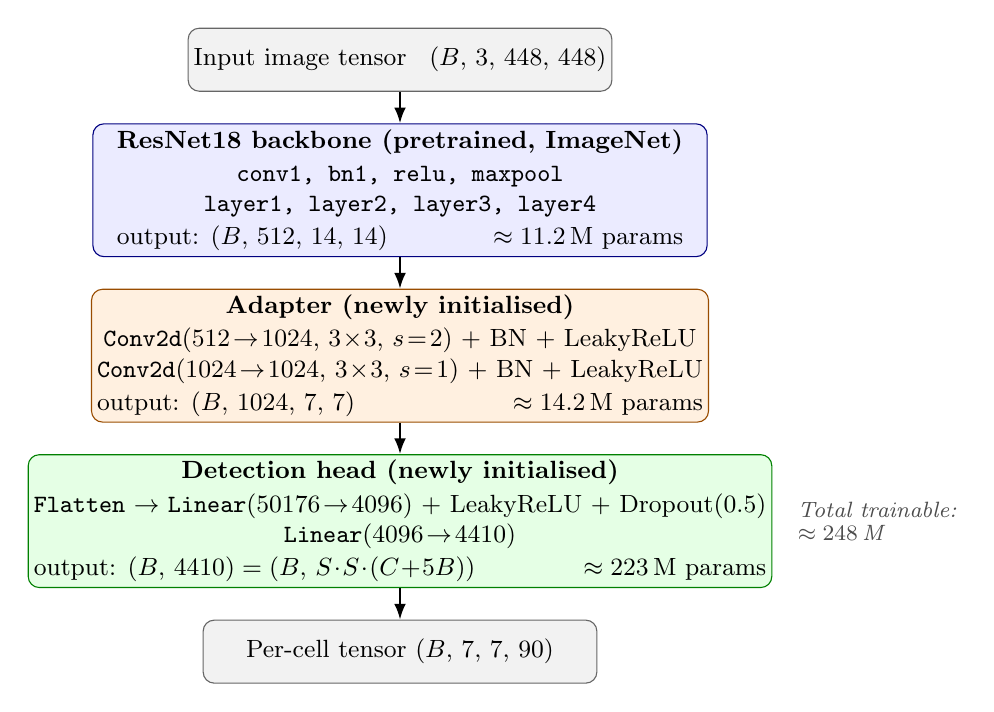
\begin{tikzpicture}[
    node distance=4mm,
    every node/.style={font=\small},
    block/.style={draw, rounded corners, align=center, minimum width=7.8cm, minimum height=8mm, inner sep=2pt},
    bb/.style    ={block, fill=blue!8,   draw=blue!50!black},
    adapter/.style={block, fill=orange!12, draw=orange!60!black},
    head/.style  ={block, fill=green!10,  draw=green!50!black},
    io/.style    ={block, fill=gray!10,   draw=black!60, minimum width=5cm},
    arr/.style   ={-{Latex[length=2mm]}, thick},
    tag/.style   ={font=\footnotesize\itshape, text=black!70}
]
% Input
\node[io] (input)  {Input image tensor $\;\;(B,\,3,\,448,\,448)$};

% Backbone block (single node, with internal text)
\node[bb, below=of input, align=center] (bb) {%
    \textbf{ResNet18 backbone (pretrained, ImageNet)}\\[1pt]
    \texttt{conv1, bn1, relu, maxpool}\\
    \texttt{layer1, layer2, layer3, layer4}\\[1pt]
    output: $(B,\,512,\,14,\,14)$ \hfill $\approx 11.2$\,M params};

% Adapter block
\node[adapter, below=of bb, align=center] (ad) {%
    \textbf{Adapter (newly initialised)}\\[1pt]
    \texttt{Conv2d}$(512\!\to\!1024,\,3\!\times\!3,\,s\!=\!2)$ + BN + LeakyReLU\\
    \texttt{Conv2d}$(1024\!\to\!1024,\,3\!\times\!3,\,s\!=\!1)$ + BN + LeakyReLU\\[1pt]
    output: $(B,\,1024,\,7,\,7)$ \hfill $\approx 14.2$\,M params};

% Head block
\node[head, below=of ad, align=center] (hd) {%
    \textbf{Detection head (newly initialised)}\\[1pt]
    \texttt{Flatten} $\to$
    \texttt{Linear}$(50176\!\to\!4096)$ + LeakyReLU + Dropout(0.5)\\
    \texttt{Linear}$(4096\!\to\!4410)$\\[1pt]
    output: $(B,\,4410) = (B,\,S\!\cdot\! S\!\cdot\! (C\!+\!5B))$ \hfill $\approx 223$\,M params};

% Reshape
\node[io, below=of hd] (out) {Per-cell tensor $(B,\,7,\,7,\,90)$};

% Arrows
\draw[arr] (input) -- (bb);
\draw[arr] (bb)    -- (ad);
\draw[arr] (ad)    -- (hd);
\draw[arr] (hd)    -- (out);

% Total params annotation
\node[tag, right=2mm of hd] {\shortstack[l]{Total trainable: \\ $\approx 248$\,M}};
\end{tikzpicture}
\caption{Architecture used in V4--V6. Blue: pretrained ResNet18 trunk loaded
from torchvision (\texttt{ResNet18\_Weights.DEFAULT}). Orange: convolutional
adapter that downsamples spatially from $14\!\times\!14$ to $7\!\times\!7$
and widens channel depth from $512$ to $1024$. Green: the two-layer fully
connected head; the first dense layer (50\,176~$\to$~4\,096) accounts for
roughly $90\,\%$ of the model's trainable parameters. The final tensor is
reshaped to $(B,\,7,\,7,\,90)$ for loss and decoding; the channel layout per
cell is the $C\!=\!80$ COCO layout defined in
Section~\ref{sec:theory:grid}.}
\label{fig:arch}
\end{figure}

\paragraph{Backbone choice.} The original YOLOv1 \citep{redmon2016you} uses a
custom 24-layer Darknet trunk pretrained on ImageNet. Reproducing this
backbone from scratch and then pretraining it on ImageNet was outside the
compute budget of this project. ResNet18 \citep{he2016deep} is the smallest
member of the residual-network family for which torchvision ships a
ready-to-use pretrained checkpoint, and its output stride and channel count
($\times 32$ downsampling, $512$ channels) match a YOLO grid of $S=7$ on a
$448 \times 448$ input. The exchange we accept is a smaller, faster,
already-pretrained trunk in exchange for a less expressive feature backbone
than the paper's; we revisit this trade-off in the Discussion.

\paragraph{Adapter.} ResNet18's \texttt{layer4} produces $(B, 512, 14, 14)$
feature maps for a $448 \times 448$ input. The detection head needs
$(B, 1024, 7, 7)$ to match the original Darknet head's expected size. The
adapter is the cheapest module that bridges the two: a stride-2 convolution
halves the spatial resolution while doubling the channel depth, and a
stride-1 convolution refines the resulting representation. Both convolutions
are followed by batch normalisation~\citep{ioffe2015batch} and a LeakyReLU
activation with negative slope $0.1$, matching the paper's choice in the
detection layers.

\paragraph{Detection head.} The head is identical to the original paper.
Flatten produces a $50\,176$-element vector, the first dense layer maps it
to $4\,096$ with LeakyReLU and dropout~\citep{srivastava2014dropout}, and the
final dense layer produces the $4\,410 = 7 \cdot 7 \cdot 90$ outputs. No
activation is applied to the final layer: the loss operates directly on the
raw logits, with no sigmoid on the box coordinates and no softmax on the
class probabilities.

\paragraph{Parameter accounting.} The first dense layer of the head accounts
for roughly $205$\,M of the $248$\,M trainable parameters
(\,$50\,176 \times 4\,096$\,). The ResNet18 trunk carries about $11.2$\,M, the
adapter contributes $\sim 14$\,M, and the remainder is split between the
final dense layer and the various biases and BN scale/offset terms. The
disparity between the convolutional trunk and the dense head is a known
weakness of the YOLOv1 design and one of the primary motivations for the
fully convolutional rewrite in YOLOv2 and YOLOv3 \citep{redmon2018yolov3}.

% -------------------------------------------------------------
\subsection{Loss implementation}
\label{sec:impl:loss}

The loss is the five-term sum-of-squared-errors formulation from
\citet{redmon2016you}. We implement it as a single \texttt{nn.Module} subclass
(\texttt{src/loss.py}) operating on per-batch tensors. A condensed listing of
the body is given in Listing~\ref{lst:loss-body}; we discuss four
implementation details that are not visible from the mathematical formulation.

\begin{lstlisting}[caption={Body of \texttt{YoloLoss.forward}, abbreviated for
brevity. Auxiliary index variables and the IoU-based responsibility mask are
omitted; the full source is in \texttt{src/loss.py}.},
label=lst:loss-body]
predictions = predictions.reshape(-1, S, S, C + 5*B)

C = self.C
OBJ_IDX    = C
BOX1_SLICE = slice(C + 1, C + 5)
CONF2_IDX  = C + 5
BOX2_SLICE = slice(C + 6, C + 10)

iou_b1   = iou(predictions[..., BOX1_SLICE], target[..., BOX1_SLICE])
iou_b2   = iou(predictions[..., BOX2_SLICE], target[..., BOX1_SLICE])
best_box = torch.max(torch.stack([iou_b1, iou_b2], dim=0), dim=0).indices

exists_box = target[..., OBJ_IDX:OBJ_IDX+1]

# Box loss (xy directly, wh under sign(.)*sqrt(|.|))
box_pred = exists_box * (best_box * predictions[..., BOX2_SLICE]
                       + (1 - best_box) * predictions[..., BOX1_SLICE])
box_tgt  = exists_box * target[..., BOX1_SLICE]

xy_pred       = box_pred[..., 0:2]
wh_pred_sqrt  = torch.sign(box_pred[..., 2:4]) * torch.sqrt(
                    torch.abs(box_pred[..., 2:4]) + 1e-6)
box_pred      = torch.cat([xy_pred, wh_pred_sqrt], dim=-1)
box_tgt       = torch.cat([box_tgt[..., 0:2],
                           torch.sqrt(box_tgt[..., 2:4] + 1e-6)], dim=-1)
box_loss  = mse(box_pred, box_tgt)

# Object + no-object + class losses (see src/loss.py for full code)
\end{lstlisting}

\paragraph{Sum reduction.} We use \texttt{nn.MSELoss(reduction="sum")} rather
than \texttt{"mean"}. The paper specifies a sum of squared errors, and the
relative weighting between the five terms is calibrated for sum reduction:
$\lambda_{\text{coord}} = 5$ is meaningful only if all of the coordinate
summands are accumulated rather than averaged. The consequence is that the
absolute loss magnitude scales with batch size and with grid density; at our
$S = 7$, $B = 2$, $C = 80$ and batch size $32$, the per-batch loss settles in
the low hundreds (as seen in V5 and V6 in
Section~\ref{sec:experiments:setup}).

\paragraph{Safe square-root on width and height.} The paper applies
$\sqrt{w}$ and $\sqrt{h}$ to equalise the gradient contribution of small and
large boxes. The network output is unconstrained, however, so any negative
prediction during early training would crash the square root. We therefore
compute $\operatorname{sign}(x) \cdot \sqrt{|x| + \varepsilon}$ with
$\varepsilon = 10^{-6}$. The sign is preserved so that the gradient through
the responsibility mask points the prediction back into the positive half-line
on the next step, rather than being trapped by an \texttt{abs} symmetry. This
trick is standard in published YOLO reimplementations but the choice of
$\varepsilon$ location matters: $\sqrt{|x| + \varepsilon}$ is safer than
$\sqrt{|x + \varepsilon|}$ near $x = -\varepsilon$.

\paragraph{Avoiding in-place writes on autograd tensors.} An earlier version
of the code transformed \texttt{box\_predictions[..., 2:4]} in place:
\begin{lstlisting}
box_predictions[..., 2:4] = torch.sign(...) * torch.sqrt(...)
\end{lstlisting}
\noindent This silently severs the autograd graph through the modified slice:
no exception is raised, the loss value is correct, but the backward pass
through the $w, h$ pathway returns zero gradients. The current implementation
re-assembles the four-component box tensor via \texttt{torch.cat} along the
channel dimension, which preserves the graph. This was fixed in the same
commit cycle as the bug investigation of
Section~\ref{sec:bug-investigation}; we mention it here because it is part of
the implementation invariants that future modifications must respect.

\paragraph{Indices derived from $C$.} As discussed at length in
Section~\ref{sec:bug:loss-indices}, the indices into the per-cell prediction
tensor are computed from \texttt{self.C} rather than hardcoded. The same
class can therefore be instantiated for any $C$ without code changes, which
both fixes the original COCO bug and keeps the class testable on the
$C\!=\!20$ VOC layout without modifications.

% -------------------------------------------------------------
\subsection{Training infrastructure}
\label{sec:impl:training}

The training loop (\texttt{src/train.py}) is written for multi-GPU operation
under PyTorch's \texttt{DistributedDataParallel} (DDP) and launched with
\texttt{torchrun}. In practice all six runs in this work used a single GPU,
but the multi-process scaffolding (process group init, distributed sampler,
rank-zero-only logging, rank-zero-only checkpointing) was retained so the
loop could be scaled later without restructuring.

\paragraph{Hardware.} V4--V6 ran on a Vast.ai pod with a single NVIDIA H200
NVL (140\,GB HBM3) and node-local NVMe storage. Throughput at $S = 7$,
$B = 2$, $C = 80$, batch size $32$ and input resolution $448\times 448$ was
approximately $114$~seconds per epoch on the training split, or
$\sim\!95$~minutes for $50$ epochs. V1--V3 ran on a different provider
(RunPod) on a pod equipped with eight NVIDIA H100 GPUs, of which only one
was effectively used because the storage substrate became the bottleneck
before compute parallelism could be exploited; the configuration is
discussed under ``Storage substrate, in passing'' below. Absolute timings
for V1--V3 are not directly comparable to V4--V6 because the backbone, the
iteration count, the GPU generation and the I/O path all differ.

\paragraph{Software stack.} PyTorch 2.4.1 with CUDA 12.4 on Python 3.12.
Mixed precision is handled by \texttt{torch.amp.autocast(device\_type="cuda",
dtype=torch.float16)} for the forward pass and the loss, with the optimiser
maintaining a float32 master copy of the weights via
\texttt{torch.amp.GradScaler}. Gradients are unscaled before clipping so that
the clip threshold is interpreted in real magnitude rather than in scaled
units.

\paragraph{Optimiser and schedule.} Stochastic gradient descent with momentum
$0.9$ and weight decay $5\!\times\!10^{-4}$, applied uniformly to every
parameter (we do not use parameter groups with a smaller learning rate on the
backbone). The schedule is a three-epoch linear warm-up from $0$ to the peak
learning rate, followed by cosine annealing to $10^{-5}$
\citep{loshchilov2017sgdr}. The peak rate is $10^{-4}$ in V4--V6 and varies
across V1--V3 as described in Section~\ref{sec:experiments:setup}.

\paragraph{Checkpoints.} The trainer writes three kinds of checkpoint per run:
a rolling \texttt{last.pth} updated every epoch, a snapshot
\texttt{epoch\_NNN.pth} every two epochs, and a \texttt{best.pth} updated only
when the validation loss strictly improves. Each ``full'' checkpoint contains
the model state dict, the optimiser state, the AMP scaler state, the epoch
number and the train/validation losses, so a run can be resumed exactly
(this is how V6 resumes from V5). For evaluation we accept both ``full''
checkpoints and ``clean'' checkpoints that are pure state dicts; the
distinction is detected by the presence of the \texttt{model\_state\_dict} key
and handled in \texttt{scripts/evaluate.py} and
\texttt{scripts/visualize\_prediction.py}.

\paragraph{Storage substrate, in passing.} An earlier attempt to host V1--V3
on a single RunPod pod equipped with $8\!\times$ NVIDIA H100 GPUs and
MooseFS-backed distributed storage was abandoned after the COCO unzip step
repeatedly placed worker processes in uninterruptible (\texttt{D}-state)
sleep, requiring pod reboots and preventing the eight-GPU configuration from
ever being exercised in a meaningful training run. The relevant lesson is
that a $26$~GB dataset of small files benefits substantially from a local
NVMe rather than a network filesystem: switching to a node-local NVMe (which
the Vast.ai pod used for V4--V6 provides natively) was the single largest
engineering improvement of the project, more impactful than any of the
architectural changes made between V1 and V4.

% -------------------------------------------------------------
\subsection{Evaluation pipeline}
\label{sec:impl:eval}

Evaluation is performed offline by \texttt{scripts/evaluate.py} against the
test split. The script loads a checkpoint, iterates over the test
\texttt{DataLoader} with \texttt{shuffle=False} (so that the bookkeeping
indices are deterministic), and for each batch performs the following steps.

\begin{enumerate}
    \item Forward pass under \texttt{torch.no\_grad}, producing the flat
        $(B, 4410)$ output tensor.
    \item Per-cell decoding via \texttt{utils.cellboxes\_to\_boxes}, which
        reshapes to $(B, 7, 7, 90)$, selects the higher-confidence of the two
        candidate boxes per cell, applies the cell-to-image coordinate
        transform discussed in Section~\ref{sec:bug:wh-decoding} (the $1/S$
        factor on $x, y$ only, post-fix), and returns a list of $49$ candidate
        boxes per image in the form
        $[\text{class},\,\text{prob},\,x,\,y,\,w,\,h]$.
    \item Per-class non-maximum suppression, parameterised by a probability
        threshold (the smallest predicted confidence to consider, set to
        $0.1$ and $0.3$ in the reported results) and an IoU threshold (the
        overlap above which a lower-confidence prediction of the same class
        is discarded, fixed at $0.5$).
    \item Aggregation of all surviving predictions across the entire test
        split into a global list of $[\text{image\_idx}, \text{class},
        \text{prob}, x, y, w, h]$ tuples.
    \item Extraction of the corresponding ground-truth list from the target
        tensors, also indexed by \texttt{image\_idx}.
    \item Computation of mean Average Precision via
        \texttt{metrics.mean\_average\_precision}, which sorts each class's
        predictions by confidence, walks them in descending order while
        marking each as a true positive (if it overlaps an unclaimed GT of
        the same class with IoU above the threshold) or false positive, and
        integrates the resulting precision--recall curve per class with the
        trapezoidal rule. The final mAP is the mean of the per-class AP over
        the 80 classes.
\end{enumerate}

\paragraph{One implementation detail.} The mAP code skips classes with zero
ground-truth instances in the evaluated split rather than counting them as
AP~$=$~0. On COCO this never triggers, because every class has at least one
test instance, but it would change the denominator if the same code were
applied to a smaller benchmark.

\paragraph{Reproducibility.} The dataset split is fixed by seed~$42$ in
\texttt{scripts/prepare\_splits.py}, the test data loader uses
\texttt{shuffle=False}, NMS is deterministic, and the loss/decoding code
contains no stochastic elements. Re-running the evaluation script on the
same checkpoint and the same hardware reproduces the reported mAP exactly.


\section{Experimentation}
\label{sec:experimentation}
% =============================================================
%  Section: Experimentation
% =============================================================

This section traces six successive training runs (V1--V6) of the YOLOv1
implementation on COCO~2017. The first four runs all produced
$\mathrm{mAP}@0.5 = 0$ on the held-out test set despite training losses that
appeared to converge. The recovery from this state of affairs is the central
narrative of this work: a sequence of hyper-parameter changes that failed to
diagnose the problem, followed by a code audit that identified two
implementation bugs invisible to the unit-test suite. V5 and V6 were trained
after the fixes and produced the first non-zero detection scores.

We adopt the convention that each version is identified by its short tag
(V1\ldots V6) and we cross-reference the corresponding row of
Table~\ref{tab:run-summary} throughout.

% -------------------------------------------------------------
\subsection{Common training setup}
\label{sec:experiments:setup}

All six versions share the optimiser, the loss formulation (whose
implementation, however, differed in V1--V4 from V5--V6 due to the bug fixes
discussed in Section~\ref{sec:bug-investigation}), the data pipeline, and the
evaluation protocol. We summarise the constants here and only describe
per-version variations in their respective subsections.

\begin{itemize}
    \item \textbf{Dataset:} COCO~2017~\citep{lin2014microsoft}, all 80 classes,
        consolidated into a single annotation file and split deterministically
        (seed $42$) into 90\,\%\,/\,5\,\%\,/\,5\,\% for train, validation and
        test. The test split contains 6\,165 images and 42\,795 ground-truth
        bounding boxes after the removal of crowd annotations. Of these, the
        dataset class retains only $31\,167$ at training time because the
        one-object-per-cell rule (Section~\ref{sec:impl:dataset}) drops any
        annotation whose grid cell is already claimed by a previously
        encountered object; the dropped boxes still count as missed
        detections at evaluation, since the evaluator reads the raw COCO
        annotations.
    \item \textbf{Optimiser:} stochastic gradient descent with Nesterov-free
        momentum~$0.9$ and weight decay~$5\!\times\!10^{-4}$, applied uniformly
        to all parameters (no parameter groups).
    \item \textbf{Learning-rate schedule:} a linear warm-up of three epochs
        from $0$ to the peak rate, followed by cosine annealing
        \citep{loshchilov2017sgdr} down to a minimum of
        $1\!\times\!10^{-5}$. The peak rate is the per-version
        parameter and is reported individually.
    \item \textbf{Mixed precision:} the forward pass runs under
        \texttt{torch.amp.autocast} in float16, while master weights and the
        loss accumulator remain in float32~\citep{micikevicius2018mixed}.
        Gradient scaling is performed with \texttt{GradScaler} and the scaled
        gradients are unscaled before clipping.
    \item \textbf{Distributed setup:} the training loop is written for
        \texttt{DistributedDataParallel} with \texttt{torchrun}, but in
        practice every run used a single GPU and a per-GPU batch size of
        $32$. V1--V3 ran on a RunPod pod equipped with $8\!\times$ NVIDIA H100
        GPUs (of which only one was effectively exercised due to the storage
        bottleneck described in Section~\ref{sec:impl:training});
        V4--V6 ran on a Vast.ai H200 NVL pod ($140$~GB HBM3) with
        node-local NVMe.
    \item \textbf{Loss:} the five-term sum-of-squared-errors loss from
        \citet{redmon2016you}, with $\lambda_{\text{coord}}=5$ and
        $\lambda_{\text{noobj}}=0.5$. The implementation is the object of
        Section~\ref{sec:bug-investigation}.
    \item \textbf{Evaluation:} the trained model is run on the full test split
        with prediction probability thresholds of $0.1$ and $0.3$, followed by
        per-class non-maximum suppression at IoU~$0.5$. The reported metric is
        mean Average Precision at IoU~$0.5$, computed per class using the
        unclaimed-GT bookkeeping described in
        Section~\ref{sec:theory:map} and averaged across the 80 classes that have at
        least one ground-truth instance in the test split (which in our case is
        all of them).
\end{itemize}

The variables that change across versions are the backbone, the peak learning
rate, the gradient clipping threshold, the number of training epochs and, most
importantly for V5 and V6, the loss and decoding code. They are summarised in
Table~\ref{tab:run-summary}.

\begin{table}[ht]
\centering
\caption{Summary of all six training runs. ``Bugs'' indicates whether the loss
and coordinate-decoding bugs analysed in Section~\ref{sec:bug-investigation}
were present at training time. Validation loss is the final per-batch
sum-reduced value from the training log; the magnitude jump between V4 and V5
is itself evidence of the bug fix and is discussed in
Section~\ref{sec:experiments:v5}.}
\label{tab:run-summary}
\small
\begin{tabular}{lllcrrcc}
\toprule
\textbf{Run} & \textbf{Backbone} & \textbf{Bugs} & \textbf{Epochs} &
\textbf{Train loss} & \textbf{Val loss} &
\textbf{mAP@0.5 (0.1)} & \textbf{mAP@0.5 (0.3)} \\
\midrule
V1 & Darknet24 & present & 33 (diverged) & --     & N/A  & 0.0000 & 0.0000 \\
V2 & Darknet24 & present & 100           & 1.45   & 1.50 & 0.0000 & 0.0000 \\
V3 & Darknet24 & present & 135           & 1.20   & 1.35 & 0.0000 & 0.0000 \\
V4 & ResNet18  & present & 50            & 0.96   & 0.98 & 0.0000 & 0.0000 \\
V5 & ResNet18  & fixed   & 50            & 336.34 & 337.37 & 0.0409 & 0.0373 \\
V6 & ResNet18  & fixed   & 60            & 330.50 & 337.40 & \textbf{0.0415} & 0.0381 \\
\bottomrule
\end{tabular}
\end{table}

% -------------------------------------------------------------
\subsection{V1: paper-faithful Darknet baseline}
\label{sec:experiments:v1}

The first attempt follows \citet{redmon2016you} as literally as the constraints
of a modern PyTorch~\citep{paszke2019pytorch} stack allow. The backbone is a
re-implementation of the paper's 24-layer Darknet, initialised from scratch
with the default PyTorch initialisation. The detection head is two fully
connected layers (50\,176~$\to$~4096~$\to$~4410) with dropout~0.5 after the
first \citep{srivastava2014dropout}. The peak learning rate is
$1\!\times\!10^{-3}$, matching the paper's choice for training from scratch on
ImageNet-free data. No gradient clipping is applied. The intended schedule is
100 epochs.

Training diverges at epoch~33: the loss tensor turns into NaN within a single
batch and remains NaN for every subsequent step. The proximate cause is the
combination of a randomly initialised 24-layer convolutional network, a
high peak learning rate, and the lack of any clipping mechanism: a single
unlucky batch produces a gradient norm large enough to push the master weights
into a region where the next forward pass overflows the fp16 dynamic range.
The run is abandoned, and no checkpoint is selected for evaluation. We
nonetheless include V1 in Table~\ref{tab:run-summary} for narrative
completeness.

% -------------------------------------------------------------
\subsection{V2: regularisation by gradient clipping}
\label{sec:experiments:v2}

V2 is a direct response to V1: the peak learning rate is halved to
$5\!\times\!10^{-4}$ and we introduce gradient-norm clipping with a threshold
of $5.0$. The architecture is unchanged. The model trains for the planned
100 epochs without divergence; the validation loss bottoms out around 1.50 and
plateaus. On the test set, however, the mAP@0.5 is still exactly zero. The
qualitative behaviour is that of a model that has learnt to drive object
confidences to almost zero everywhere: post-NMS detections are scarce and
their bounding boxes are unrelated to the ground-truth objects.

We interpreted this at the time as a sign that the lowered learning rate was
preventing the network from escaping a trivial minimum of the no-object
confidence term. In hindsight, this interpretation was incomplete: the
``trivial minimum'' was indeed real, but its existence was caused by the loss
bug discussed in Section~\ref{sec:bug:loss-indices}, not by the
hyper-parameters.

% -------------------------------------------------------------
\subsection{V3: relaxing the clip, restoring the LR}
\label{sec:experiments:v3}

V3 returns the peak learning rate to $1\!\times\!10^{-3}$ and increases the
gradient-clip threshold to $10.0$, with the working hypothesis that V2 was
under-trained. The number of epochs is extended to 135 to match the paper's
total schedule length. The training loss continues to decrease and reaches its
lowest value across the Darknet runs (1.20), but the validation loss begins to
diverge from training loss around epoch~$\sim 40$, which we interpreted as
overfitting. mAP@0.5 on the test set is again exactly zero.

At this point the working hypothesis became that the Darknet backbone, trained
from scratch on COCO without the ImageNet pre-training stage that
\citet{redmon2016you} performed, simply lacks the inductive bias needed for
this dataset. We therefore moved on to V4.

% -------------------------------------------------------------
\subsection{V4: ResNet18 pretrained on ImageNet}
\label{sec:experiments:v4}

V4 replaces the 24-layer Darknet with a ResNet18~\citep{he2016deep} loaded with
ImageNet weights from \texttt{torchvision} (\texttt{ResNet18\_Weights.DEFAULT}).
The classification head of the ResNet is discarded and the convolutional trunk
up to and including \texttt{layer4} produces feature maps of shape
$(B, 512, 14, 14)$ given the standard $448\times 448$ input. We bridge to the
detection head's expected $(B, 1024, 7, 7)$ with a two-layer adapter (a
stride-2 convolution from $512$ to $1024$ channels, followed by a stride-1
convolution that refines the representation), each with batch
normalisation~\citep{ioffe2015batch} and a LeakyReLU activation. The detection
head is identical to V1--V3. All parameters of the model carry
\texttt{requires\_grad=True} from epoch one; we do not freeze any layer.

Because the backbone now expects ImageNet-normalised inputs, the dataset
transform is augmented with the standard channel mean/std normalisation. The
peak learning rate is reduced to $1\!\times\!10^{-4}$ to fine-tune the
pretrained convolutional features without destroying them, while still leaving
enough learning capacity for the randomly initialised adapter and FC head
(which between them carry the majority of the model's 248~M parameters).
Gradient clipping is kept at $10.0$, and the schedule is shortened to 50
epochs.

V4 trains without numerical issues. The validation loss reaches 0.98 at the
best epoch---the lowest value yet, and on its face suggestive of a model that
has fit the data well. Yet the mAP@0.5 on the test set is again exactly zero.
Post-NMS we observe a different qualitative failure mode from V2/V3: the
model emits a large number of low-confidence boxes per image (on the order
of 20 with $p > 0.005$), but they are spatially uncorrelated with the ground
truth, and their predicted classes do not match.

This was the result that forced the question: \emph{is the loss decreasing
because the model is learning, or because it is finding a trivial minimum of a
loss that is not what we think it is}? The investigation that followed is the
subject of the next section.

% =============================================================
\subsection{Bug investigation}
\label{sec:bug-investigation}

The trigger for an audit was the observation that, across four runs with very
different hyper-parameter settings and two different backbones, the test mAP
remained identically zero while the validation losses spanned the range
$0.96$--$1.50$. A loss that decreases consistently across hyper-parameter
sweeps but produces a detector that detects nothing is suspect: either the
model genuinely has no localisation capacity in this regime (which is hard to
reconcile with a fully fine-tuned ResNet18 at val\_loss~$<\!1$), or the loss is
not enforcing the constraint we expect.

The audit identified two independent bugs, each of which is sufficient on its
own to produce $\mathrm{mAP}@0.5 = 0$. The first is in the loss function; the
second is in the post-processing routine that converts model outputs back to
image-relative bounding boxes. We discuss them in turn.

% -------------------------------------------------------------
\subsubsection{Bug~1: VOC-layout indices applied to COCO tensors}
\label{sec:bug:loss-indices}

The original implementation of the YOLO loss in \texttt{src/loss.py} addressed
the per-cell prediction tensor by hardcoded integer indices that matched the
Pascal VOC layout (20 classes, $C=20$). The expected per-cell layout for
$C=20$ is
\[
  \underbrace{[\,0,\;\ldots,\;19\,]}_{\text{class probabilities}}\;\;
  \underbrace{[\,20\,]}_{\text{conf}_1}\;\;
  \underbrace{[\,21,\;\ldots,\;24\,]}_{x_1,\,y_1,\,w_1,\,h_1}\;\;
  \underbrace{[\,25\,]}_{\text{conf}_2}\;\;
  \underbrace{[\,26,\;\ldots,\;29\,]}_{x_2,\,y_2,\,w_2,\,h_2},
\]
which the loss reads literally as \texttt{[..., 20:21]} for the
``object exists'' mask, \texttt{[..., 21:25]} for the first predicted box, and
so on. For COCO with $C=80$, the actual per-cell tensor produced by the
dataset is
\[
  \underbrace{[\,0,\;\ldots,\;79\,]}_{\text{class probabilities}}\;\;
  \underbrace{[\,80\,]}_{\text{conf}_1}\;\;
  \underbrace{[\,81,\;\ldots,\;84\,]}_{x_1,\,y_1,\,w_1,\,h_1}\;\;
  \underbrace{[\,85\,]}_{\text{conf}_2}\;\;
  \underbrace{[\,86,\;\ldots,\;89\,]}_{x_2,\,y_2,\,w_2,\,h_2},
\]
so the indices used by the loss point inside the \emph{class probability}
region of the tensor, never reaching the coordinate slots.

The downstream consequences are catastrophic, but each consequence is locally
silent:
\begin{enumerate}
    \item \texttt{target[..., 20:21]}, which the loss interprets as the
        object-presence indicator (\texttt{exists\_box}), is in COCO the
        class-probability slot for class index~20 (which after the dense COCO
        remapping is the \emph{elephant} class). The mask is therefore $1$
        only in cells whose ground-truth class is elephant, and $0$ otherwise.
    \item The coordinate slots that the loss reads
        (\texttt{predictions[..., 21:25]}, \texttt{target[..., 21:25]}) are
        actually class probability slots for class indices~21--24
        (\emph{bear}, \emph{zebra}, \emph{giraffe}, \emph{backpack}). The IoU
        computation between two slices of class probabilities returns a
        nonsense quantity that is essentially uncorrelated with anything the
        network can learn from.
    \item The class loss is computed over the slice
        \texttt{predictions[..., :20]}, so only the first twenty COCO classes
        (out of eighty) participate in the class term at all. Classes 20--79
        receive no gradient signal whatsoever.
    \item The no-object loss penalises \texttt{predictions[..., 20]} and
        \texttt{predictions[..., 25]} in cells where the target's position~20
        is zero. Position~20 of the target is zero in the overwhelming
        majority of cells (those that do not happen to contain an elephant),
        so the model is strongly pulled towards driving these two output
        positions to zero everywhere. Position~20 and~25 in the prediction
        tensor, however, are not the confidence slots; they are the
        class-probability slots for the class \emph{elephant} and (in
        practice, after \texttt{argmax}) the slot interpreted as ``conf~2''
        is the class probability for \emph{train}. The trivial-minimum
        behaviour observed in V2--V4 is a faithful learning of this confused
        no-object signal, not a property of the MSE loss as such.
\end{enumerate}

The bug is invisible from a unit-testing perspective. The existing test in
\texttt{tests/test\_loss.py} instantiates the loss with $C=20$:

\begin{lstlisting}[caption={Pre-fix unit test that passed for the wrong reason.},label=lst:voc-test]
loss_fn = YoloLoss(S=7, B=2, C=20)
target = torch.zeros(1, 7, 7, 30)
target[0, 3, 4, 0]    = 1                              # class
target[0, 3, 4, 20]   = 1                              # confidence
target[0, 3, 4, 21:25] = torch.tensor([0.5, 0.5, 0.3, 0.3])
\end{lstlisting}

\noindent At $C=20$, the indices $20$, $21\!:\!25$, $25$, $26\!:\!30$ that the
loss reads happen to coincide with the slots that the dataset writes, so the
test passes. The test would have to be parametrised on $C$ to detect the
mismatch; ours was not.

\paragraph{Verification.} We constructed a synthetic COCO-shaped target with
one ground-truth object at class~7, cell~$(3,4)$, with box
$(x_c, y_c, w, h) = (0.5, 0.5, 0.3, 0.3)$ and computed the loss on two
predictions:

\begin{enumerate}
    \item A ``perfect'' prediction that matches the target at all slots,
        including the correct COCO coordinate slots $[81\!:\!85]$.
    \item The same prediction but with the four box-coordinate slots
        $[81\!:\!85]$ overwritten with arbitrarily large values
        ($99.0,\ldots,99.0$).
\end{enumerate}

Under a correctly indexed loss, prediction~(2) must produce a much larger
value than prediction~(1). Under the buggy loss, the two values were
identical to within numerical precision: $0.000490$ in both cases. This
confirms that the loss was \emph{gradient-blind} to the slots that the model
is supposed to predict.

Aggregated over a sample of 200 real COCO training images, the buggy
$\texttt{exists\_box}$ mask was $1$ in only 3 cells out of $1\,062$ cells that
actually contained a ground-truth object---about $0.3\,\%$---and these three
were all elephants. The remaining $99.7\,\%$ of real objects contributed
exactly zero to the box and object terms of the loss.

\paragraph{Fix.} We replaced every hardcoded literal in the loss with an index
derived from \texttt{self.C}:

\begin{lstlisting}[caption={Index variables introduced at the top of
    \texttt{YoloLoss.forward}.}]
C          = self.C
OBJ_IDX    = C
BOX1_SLICE = slice(C + 1, C + 5)
CONF2_IDX  = C + 5
BOX2_SLICE = slice(C + 6, C + 10)
\end{lstlisting}

\noindent and propagated these names through every site that previously held a
literal. The class term was also corrected from
\texttt{predictions[..., :20]} to \texttt{predictions[..., :C]} so that all 80
classes participate. The pre-existing $C=20$ unit test continues to pass
because the new variables evaluate to the same numeric positions when $C=20$.
A full side-by-side diff is provided in Appendix~\ref{app:loss-diff}.

A second, smaller follow-up to the loss was committed shortly afterwards: the
square-root transform of $w$ and $h$ (the paper's trick to equalise the
contribution of small and large boxes) was implemented as an \emph{in-place}
assignment, \texttt{box\_predictions[..., 2:4] = \ldots}. In-place writes on a
tensor that participates in the autograd graph silently sever the backward
pass through that tensor, with no exception raised at runtime. The fix is to
re-assemble the modified tensor with \texttt{torch.cat} along the channel
dimension. We mention this here for completeness; it did not affect the V1--V4
runs because, given Bug~1, no gradient flowed through that path anyway.

% -------------------------------------------------------------
\subsubsection{Bug~2: spurious \texorpdfstring{$1/S$}{1/S} factor in \texorpdfstring{$w,\,h$}{w, h} decoding}
\label{sec:bug:wh-decoding}

The post-processing routine \texttt{convert\_cellboxes} in
\texttt{src/utils.py} converts the raw per-cell prediction tensor into a list
of bounding boxes in image-relative coordinates. The conversion of the
$(x, y)$ centre coordinates is straightforward: the predictions are stored as
offsets within the cell, so the global $x$ coordinate is the cell column index
plus the in-cell offset, divided by $S$:
\[
  x_{\text{global}} = \frac{j + x_{\text{cell}}}{S}, \qquad
  y_{\text{global}} = \frac{i + y_{\text{cell}}}{S}.
\]
The width and height, however, are stored by the dataset as ratios of the
\emph{whole image} dimensions ($w_{\text{norm}} = w_{\text{px}}/W_{\text{img}}$
and likewise for $h$), and the loss compares the model's $w,h$ output
\emph{directly} against these values. The model therefore learns to predict
$w_{\text{norm}}, h_{\text{norm}}$.

In our implementation the decoding code, however, performed an additional
division by $S$:
\begin{lstlisting}
w_h = (1.0 / S) * best_boxes[..., 2:4]   # BUG: divides w,h by 7
\end{lstlisting}

\noindent This is the symmetric mistake of porting from a different
encoding. The implementation we drew partial inspiration
from~\citep{persson2020yolo} stores width and height as $w_{\text{norm}}\cdot S$
and $h_{\text{norm}}\cdot S$ (``number of cells the box spans''), so dividing
by $S$ at decode time is correct \emph{in that codebase}. In ours it is not.

\paragraph{Consequence.} Every predicted box is decoded with width and height
seven times smaller than the value the model has learnt to output. Given that
the network was trained to predict $w_{\text{norm}}, h_{\text{norm}} \in [0,1]$,
this scaling produces boxes of at most one-seventh of the correct linear
dimension and roughly one-forty-ninth of the correct area.

The arithmetic upper bound on the IoU between such a shrunken prediction and
its perfectly aligned ground truth is
\[
  \text{IoU} \le \frac{(\tfrac{1}{S})^2}{1 + (\tfrac{1}{S})^2 - (\tfrac{1}{S})^2}
              = \frac{1}{S^2} \approx 0.020,
\]
which is far below the threshold of $0.5$ used in mAP@0.5. The bug is
therefore sufficient on its own to drive the metric to exactly zero, even in
the hypothetical scenario where the loss bug had not also existed and the
network had learnt to localise objects correctly.

\paragraph{Verification.} We encoded a known box with $w=h=0.3$ centred at
cell~$(3,3)$, passed the tensor through \texttt{convert\_cellboxes}, and
inspected the decoded width and height. The buggy code returned
$w_{\text{dec}} = h_{\text{dec}} = 0.0429$, which is exactly $0.3/7$, while
$x$ and $y$ round-tripped correctly. After removing the $1/S$ factor on
$w_h$, the round-trip is exact to floating-point precision.

\paragraph{Fix.} The fix is one line: drop the $1/S$ factor on $w_h$ while
keeping it on $x$ and $y$. Variable renamed from \texttt{w\_y} to \texttt{w\_h}
for clarity.

% -------------------------------------------------------------
\subsubsection{Why the unit-test suite did not catch either bug}
\label{sec:bug:tests}

Both bugs are detectable with a single round-trip check, but the existing test
suite covered shapes and value ranges only. The pre-existing tests for
\texttt{convert\_cellboxes} were:
\begin{itemize}
    \item \texttt{test\_convert\_cellboxes\_output\_shape}: asserts the output
        is of shape $(B, S^2, 6)$.
    \item \texttt{test\_convert\_cellboxes\_class\_indices\_in\_range}: asserts
        that the predicted class index column lies in $[0, C-1]$.
\end{itemize}

\noindent Neither inspects the value of $w, h$. A test of the form ``encode a
known box, decode it, assert that the recovered $w, h$ match'' would have
detected Bug~2 trivially. Likewise, a loss test parameterised on $C$ with
$C \in \{20, 80\}$ would have detected Bug~1 on the very first run: the
``perfect prediction'' test at $C=80$ would have returned a non-zero loss for
any prediction whose values at the bogus VOC slots did not happen to coincide
with the class probabilities at those slots. We added both round-trip tests
together with the fixes, as documented in
Section~\ref{sec:experiments:v5}.

\paragraph{Generalisable lesson.} The deeper failure here is not the specific
indices but the assumption that a unit test that compiles, runs and passes
is evidence that the function it tests is correct. The two tests above did
exactly what they claimed and provided zero evidence about the function's
mathematical correctness. In a detection pipeline, where intermediate tensors
have many slots and most of them are unused by any single test image, the
density of meaningful coverage per unit test is low. The round-trip checks
we added pin down a single quantitative invariant per function and break
when the function's mathematical contract changes, which is the level of
specificity that is missing from shape-only assertions.

% -------------------------------------------------------------
\subsection{V5: applying the fixes}
\label{sec:experiments:v5}

V5 retains every hyper-parameter from V4---the same ResNet18 backbone, the
same adapter, the same FC head, the same peak learning rate of
$1\!\times\!10^{-4}$, the same gradient-clip threshold of $10.0$, the same
50-epoch schedule, the same optimiser, batch size and warm-up
configuration---and changes only the loss and decoding code as described in
Section~\ref{sec:bug-investigation}. The point of holding everything else
equal is to attribute any change in the result to the fixes alone.

The first observation, available from the very first epoch of training, is
that the magnitude of the loss is now in a completely different regime.
Whereas V4 produced training and validation losses around $0.96$--$0.98$, V5
produces values in the range of several hundred. The final training and
validation losses are $336.34$ and $337.37$ respectively. We had expected this:
the loss is reduced with \texttt{nn.MSELoss(reduction="sum")} over all 90
slots of every cell of every image in a batch. In V1--V4, due to Bug~1, almost
all the per-cell summands collapsed to zero, because they were multiplied by
the ``exists\_box'' mask which was itself zero almost everywhere. The
non-trivially zero contributions came almost entirely from a few elephant
cells. Once the indices are corrected, every cell with an object contributes
to the box and confidence terms, and every cell contributes to the no-object
term and the class term. The absolute magnitude of the loss therefore rises
by two orders of magnitude. This is not a regression; it is the loss finally
seeing the data.

At evaluation time, V5 produces $\mathrm{mAP}@0.5 = 0.0409$ at
prob\_threshold~$0.1$ on the test set, and $0.0373$ at prob\_threshold~$0.3$
(see Table~\ref{tab:run-summary}). This is the first non-zero detection score
of the entire project. It is a low absolute number---we discuss in detail in
Section~\ref{sec:results} why this is so, and in the Discussion section what
would be required to push it higher---but it is a categorical change from the
preceding four runs.

The qualitative behaviour also changes. Detection boxes now cluster on actual
objects in the scene, predicted classes correlate with ground-truth classes on
the easy classes (animals with distinctive silhouettes, vehicles), and per-NMS
detection counts drop to a sensible 2--6 boxes per image at
prob\_threshold~$0.3$. We provide examples drawn from the test set, sorted by
qualitative quality, in Section~\ref{sec:results}.

% -------------------------------------------------------------
\subsection{V6: continuation of V5}
\label{sec:experiments:v6}

V6 is a continuation of V5 rather than a separate experiment. We resumed
training from the V5 ``best'' checkpoint and trained for an additional 10
epochs, holding every other setting identical. The motivation was to verify
that the V5 result was not a coincidence of the cosine schedule landing on a
favourable epoch, and to give the model a bit more time near the bottom of the
learning rate ramp.

The final validation loss is essentially identical to V5 (337.40 vs.\ 337.37),
indicating that the schedule has reached saturation. The test mAP improves
marginally to $0.0415$ at prob\_threshold~$0.1$ and $0.0381$ at $0.3$. We treat
V6 as the headline run of the project and use its checkpoint
(\texttt{v6\_run/best\_v6.pth}) for all subsequent analyses in
Section~\ref{sec:results}, including the full per-class AP table in
Appendix~\ref{app:per-class-ap} and the qualitative figures.

% -------------------------------------------------------------
\subsection{Loss curves and a note on the magnitude shift}
\label{sec:experiments:curves}

Figure~\ref{fig:loss-curves} plots the training and validation loss curves
across V4, V5 and V6 on a shared time axis. The visual jump in absolute
magnitude between V4 and V5 is the empirical signature of the index fix. The
right panel zooms in on V5+V6 to make the slow descent of both training and
validation losses visible at the appropriate scale.

\begin{figure}[!ht]
\centering

\includegraphics[width=0.95\textwidth]{loss_comparison_v3.png}
\caption{Training and validation loss across runs. Left: V4 (bugs present)
plateauing near $1.0$. Middle: V5+V6 (fixes applied) plateauing near $337$.
Right: zoom on the last ten epochs of V5+V6, showing the slow improvement that
the absolute scale makes invisible in the middle panel. The magnitude jump
between V4 and V5 is itself the signature of the bug fix discussed in
Section~\ref{sec:bug-investigation}.}
\label{fig:loss-curves}
\end{figure}

A reader who reaches V5 in the training log without the context of
Section~\ref{sec:bug-investigation} could reasonably mistake the rise in loss
for a regression. We emphasise that the comparison between V4 and V5 is a
comparison between two losses that compute fundamentally different
quantities, not between a well-trained and a poorly-trained version of the
same loss.


\section{Results}
\label{sec:results}
% =============================================================
%  Section: Results
% =============================================================

The results in this section are computed on the held-out COCO test split (5\,\%
of the consolidated dataset, $6\,165$ images, $42\,795$ ground-truth bounding
boxes after the removal of crowd annotations; cf.\ the discussion of the
one-object-per-cell drop in Section~\ref{sec:experiments:setup}). All
numbers correspond to the V6 checkpoint (\texttt{v6\_run/best\_v6.pth})
introduced in Section~\ref{sec:experiments:v6}. Inference uses per-class non-maximum
suppression with an IoU threshold of $0.5$ and is run at two prediction
probability thresholds, $0.1$ (permissive) and $0.3$ (stricter), in order to
characterise the precision/recall trade-off rather than commit to a single
operating point.

% -------------------------------------------------------------
\subsection{Headline metric}
\label{sec:results:headline}

Table~\ref{tab:headline} reports the mean Average Precision at IoU~$0.5$
(mAP@0.5) on the COCO test split for both probability thresholds. The
headline number for the project, used in the abstract and the conclusions, is
$\mathrm{mAP}@0.5 = 0.0415$ at probability threshold~$0.1$.

\begin{table}[!ht]
\centering
\caption{Final detection metrics of the V6 checkpoint on the COCO test split.
Averaged over the 80 COCO classes, all of which have at least one ground-truth
instance in the test split.}
\label{tab:headline}
\small
\begin{tabular}{lcc}
\toprule
\textbf{Probability threshold} & \textbf{mAP@0.5} & \textbf{Number of classes with AP $>$ 0} \\
\midrule
0.1 & \textbf{0.0415} & 60 / 80 \\
0.3 & 0.0381          & 58 / 80 \\
\bottomrule
\end{tabular}
\end{table}

\noindent We make no claim of competitiveness with current detectors; the
purpose of the figure is to bound the absolute performance of a paper-faithful
YOLOv1 implementation, re-targeted to COCO with a ResNet18 backbone, trained
for $\sim 60$ epochs in total on a single GPU. The remainder of this section
is dedicated to characterising \emph{where} the model spends and fails to
spend that detection budget.

% -------------------------------------------------------------
\subsection{Per-class breakdown}
\label{sec:results:perclass}

Of the 80 COCO classes evaluated at threshold~$0.1$, the AP distribution is
strongly skewed: the top decile (eight classes) accounts for the bulk of the
mAP value, while a long tail of twenty classes registers exactly zero. The
full ranked table for both thresholds is provided in
Appendix~\ref{app:per-class-ap}; we discuss the structure of the distribution
here.

\paragraph{Top performers.} Table~\ref{tab:top10} lists the ten classes with
the highest AP at probability threshold~$0.1$. The pattern is consistent:
classes with large, structurally distinctive silhouettes
(zebra stripes, giraffe necks, elongated train and airplane fuselages) and
classes that tend to be photographed as the main subject of the image
(cat, bear, elephant, bus) dominate the head of the distribution.

\begin{table}[!ht]
\centering
\caption{Top-10 classes by AP@0.5 (V6, threshold~$0.1$). The ``GT in test''
column is the number of ground-truth instances of the class in the test
split.}
\label{tab:top10}
\small
\begin{tabular}{lrrr}
\toprule
\textbf{Class} & \textbf{AP@0.5} & \textbf{GT in test} & \textbf{Class idx} \\
\midrule
zebra      & 0.3593 &  236 & 22 \\
train      & 0.3265 &  212 &  6 \\
giraffe    & 0.3107 &  225 & 23 \\
cat        & 0.2575 &  255 & 15 \\
airplane   & 0.1857 &  238 &  4 \\
pizza      & 0.1795 &  257 & 53 \\
bear       & 0.1698 &   67 & 21 \\
elephant   & 0.1634 &  223 & 20 \\
bus        & 0.1595 &  246 &  5 \\
toilet     & 0.1435 &  237 & 61 \\
\bottomrule
\end{tabular}
\end{table}

\paragraph{Classes with $\mathrm{AP}=0$.} At threshold~$0.1$, twenty COCO
classes register zero detections that pass mAP's IoU criterion. Inspecting
this set reveals four distinct failure modes, each of which is consistent with
the documented weaknesses of YOLOv1~\citep{redmon2016you} and is amplified by
our particular setting.

\begin{itemize}
    \item \emph{Objects smaller than one grid cell.} With $S=7$ and an input
        resolution of $448\times 448$ pixels, each grid cell covers a
        $64\times 64$ patch of the image. Toothbrushes, hair driers, scissors
        and remote controls occupy substantially less than this footprint in
        a typical photograph. YOLOv1's ``one object per cell'' constraint
        means the detection head has no way to localise multiple sub-cell
        objects, and the regression target for the single object it does
        attempt to localise is dominated by quantisation noise.
    \item \emph{Thin or elongated tableware in cluttered scenes.} Fork,
        knife, spoon and hot dog all appear most frequently in dining table
        and food-tray scenes where many of them are grouped within a single
        cell. The same constraint applies: only one of them can be
        ``responsible'' per cell.
    \item \emph{Rare classes.} Hair drier (5 GT in the test split), toaster
        (9), parking meter (59), scissors (78), toothbrush (80) and stop sign
        (76) have so few training instances that the model has had limited
        opportunity to learn a robust template for them. The exception in the
        top performers, bear (67 GT), shows that rarity alone is not
        sufficient to drive AP to zero; rarity \emph{combined with} a small
        or non-distinctive silhouette is.
    \item \emph{Sports objects in cluttered foregrounds.} Sports ball,
        frisbee, baseball bat, baseball glove and snowboard typically appear
        in scenes dominated by human figures with the object partially
        occluded or near the image periphery. The class loss for the
        responsible cell is therefore in direct competition with the much
        stronger gradient from the co-located ``person'' instance.
\end{itemize}

\paragraph{The frequency--AP decoupling.} A naive expectation is that AP
should grow monotonically with the number of ground-truth instances seen
during training. The data refutes this clearly. The ``person'' class is the
most common in COCO by a wide margin (8\,779 GT instances in the test split,
roughly 17\,\% of all annotations) and attains only $\mathrm{AP}=0.035$. The
``car'' class (1\,382 GT) attains $0.005$. ``Chair'' (1\,336 GT) attains
$0.002$. Conversely, zebra and giraffe, with under 240 instances each, are at
the top. The discriminating factor is not frequency but a combination of size,
distinctiveness and image context.

\paragraph{Effect of the probability threshold.} Moving from threshold~$0.1$
to $0.3$ drops the mAP by approximately $8\,\%$ (from $0.0415$ to $0.0381$).
Most of the absolute loss comes from classes whose model output is uncertain
even when correct: \emph{zebra} loses $2.2$ percentage points of AP and
\emph{giraffe} $1.2$ percentage points, while \emph{train} is essentially
unaffected ($-0.2$ points). The set of zero-AP classes grows by two
(\emph{mouse} and \emph{cell phone}, both flipping from $\sim\!10^{-4}$ to
$0$). The shift is consistent with a calibration in which true positives
at this stage of training are concentrated near the lower confidence values
rather than the higher ones.

% -------------------------------------------------------------
\subsection{Qualitative analysis}
\label{sec:results:qualitative}

We illustrate the model's behaviour with examples drawn from the test split.
The selection is partitioned into three subjective categories: \emph{good}
(every ground-truth object is detected with a class-correct, well-localised
box and few false positives), \emph{medium} (the primary subject is
recognised but localisation is imperfect or one of several objects is missed)
and \emph{bad} (the prediction is essentially uncorrelated with the
ground truth, or the only detected box is a false positive of a different
class).

\begin{figure}[!ht]
\centering
\begin{subfigure}[t]{0.32\textwidth}
    
\includegraphics[width=\linewidth]{pred_015522_best_v6.png}
    \caption{Multiple distinct subjects.}
\end{subfigure}\hfill
\begin{subfigure}[t]{0.32\textwidth}
    
\includegraphics[width=\linewidth]{pred_059397_best_v6.png}
    \caption{Single subject, tight box.}
\end{subfigure}\hfill
\begin{subfigure}[t]{0.32\textwidth}
    
\includegraphics[width=\linewidth]{pred_089898_best_v6.png}
    \caption{High-AP class on a clean background.}
\end{subfigure}
\caption{Good detections (V6 checkpoint, probability threshold~$0.3$). The
common factor across the good set is a large, centrally placed subject from
one of the head classes of the distribution analysed in
Section~\ref{sec:results:perclass}.}
\label{fig:preds-good}
\end{figure}

\begin{figure}[!ht]
\centering
\begin{subfigure}[t]{0.32\textwidth}
    
\includegraphics[width=\linewidth]{pred_001560_best_v6.png}
    \caption{Localisation drifts off the subject.}
\end{subfigure}\hfill
\begin{subfigure}[t]{0.32\textwidth}
    
\includegraphics[width=\linewidth]{pred_016274_best_v6.png}
    \caption{Class correct, secondary object missed.}
\end{subfigure}\hfill
\begin{subfigure}[t]{0.32\textwidth}
    
\includegraphics[width=\linewidth]{pred_079617_best_v6.png}
    \caption{Box too large for the object.}
\end{subfigure}
\caption{Medium-quality detections. The detector identifies the dominant
object in the scene but with imperfect localisation, or misses secondary
objects whose centres fall in cells already claimed by another instance.}
\label{fig:preds-medium}
\end{figure}

\begin{figure}[!ht]
\centering
\begin{subfigure}[t]{0.32\textwidth}
    
\includegraphics[width=\linewidth]{pred_000001_best_v6.png}
    \caption{Class confusion.}
\end{subfigure}\hfill
\begin{subfigure}[t]{0.32\textwidth}
    
\includegraphics[width=\linewidth]{pred_026429_best_v6.png}
    \caption{No detection above threshold.}
\end{subfigure}\hfill
\begin{subfigure}[t]{0.32\textwidth}
    
\includegraphics[width=\linewidth]{pred_062225_best_v6.png}
    \caption{Cluttered scene with small objects.}
\end{subfigure}
\caption{Failure cases. Either the prediction is of a different class than
the ground truth (left), no prediction survives the probability filter
(middle), or the scene contains small objects below the effective resolution
of the $S=7$ grid (right).}
\label{fig:preds-bad}
\end{figure}

The qualitative split corroborates the per-class analysis: every example in
the good set features a single dominant subject from a head class, the medium
set fails on either secondary objects or imprecise localisation, and the bad
set is dominated by small-object and cluttered-scene cases. We did not curate
the bad examples to avoid the head classes; the bad failures simply occur
mostly outside the head.

% -------------------------------------------------------------
\subsection{Inference latency}
\label{sec:results:latency}

Although YOLOv1's original motivation was real-time inference, latency is not
the centrepiece of this work, because the training-time bug investigation in
Section~\ref{sec:bug-investigation} dominates the contribution. For
completeness, we report the forward-pass latency of the V6 checkpoint measured
by \texttt{scripts/realtime\_detect.py} in its \texttt{-{}-benchmark} mode,
which runs the model on synthetic batch-size-1 inputs after a warm-up and
records the per-call wall-clock time with explicit
\texttt{torch.cuda.synchronize} barriers before and after each forward pass.

\begin{table}[!ht]
\centering
\caption{Forward-only inference latency of the V6 model on an NVIDIA
GeForce RTX~5070~Ti~Laptop, batch size~1, $448\!\times\!448$ input. Statistics
over 50 timed iterations after a 20-iteration warm-up. Peak GPU memory
allocated: $\sim\!1.9$~GB.}
\label{tab:latency}
\small
\begin{tabular}{lrr}
\toprule
\textbf{Statistic} & \textbf{Latency (ms)} & \textbf{Throughput (FPS)} \\
\midrule
mean         & 5.32 & 188.1 \\
median       & 5.24 & 190.9 \\
$p_{95}$     & 6.27 & 159.5 \\
$p_{99}$     & 6.76 & 147.9 \\
\bottomrule
\end{tabular}
\end{table}

\noindent The model comfortably exceeds the real-time threshold typically
associated with the original paper, which reports 45~FPS for the base YOLO
model on a Titan~X. The gap is mostly explained by hardware
(an Ada-generation laptop GPU vs.\ a 2016-era Titan~X), not by the
architecture: the parameter count of our model (248~M) is in fact larger than
the paper's, but it is dominated by a single dense layer whose evaluation is
trivial on modern hardware. When the same script is run in its interactive
webcam mode---which adds frame capture, BGR$\to$RGB conversion, NMS, drawing
and a GUI window to the inference loop---throughput is correspondingly lower
and limited primarily by the webcam's frame-rate cap.

% -------------------------------------------------------------
\subsection{Comparison with the original paper}
\label{sec:results:vs-paper}

Table~\ref{tab:vs-paper} contrasts the configuration and headline result of
this work with the figures reported by \citet{redmon2016you}. The two are not
directly comparable as benchmarks---the datasets differ (COCO vs Pascal~VOC)
and so do the backbones and training budgets---but the comparison is useful
to bound the order-of-magnitude gap and to make explicit which contributing
factors are deliberate (dataset, backbone) and which are pragmatic (training
length, augmentation budget).

\begin{table}[!ht]
\centering
\caption{Side-by-side comparison with the original YOLOv1 paper.}
\label{tab:vs-paper}
\small
\begin{tabular}{lll}
\toprule
\textbf{Aspect} & \textbf{\citet{redmon2016you}} & \textbf{This work (V6)} \\
\midrule
Dataset                & VOC 2007 + 2012 (20 classes)   & COCO 2017 (80 classes) \\
Backbone               & Darknet24 (custom)             & ResNet18 (pretrained) \\
Backbone pretraining   & Manual on ImageNet             & torchvision IMAGENET1K\_V1 \\
Peak learning rate     & $10^{-2}$ (manual schedule)    & $10^{-4}$ \\
LR schedule            & Manual ($10^{-3}\!\to\!10^{-2}\!\to\!10^{-3}\!\to\!10^{-4}$) & Linear warm-up + cosine \\
Epochs                 & 135                             & 60 (V5 + V6 combined) \\
Batch size             & 64                              & 32 \\
Input resolution       & $448\times 448$                 & $448\times 448$ \\
Grid ($S$)             & 7                               & 7 \\
Boxes per cell ($B$)   & 2                               & 2 \\
Output channels per cell & $20 + 5\cdot 2 = 30$         & $80 + 5\cdot 2 = 90$ \\
Augmentation           & Crops, exposure, saturation, scaling & Resize only \\
$\lambda_{\text{coord}}$ & 5                            & 5 \\
$\lambda_{\text{noobj}}$ & 0.5                          & 0.5 \\
Hardware               & NVIDIA Titan~X (2016)          & NVIDIA H200~NVL (2024) \\
Wall-clock training    & $\sim$ 1 week                  & $\sim$ 2 hours \\
\midrule
\textbf{mAP@0.5}       & 63.4 (VOC 2007 test)            & 4.15 (COCO test, threshold~0.1) \\
\bottomrule
\end{tabular}
\end{table}

\noindent The gap of roughly $\times 15$ in headline mAP is dominated by four
factors that we discuss in detail in the Discussion: (i) COCO is a
substantially harder benchmark than VOC, both in terms of class count and in
terms of object size distribution, (ii) the original paper trains for more
than twice as long, (iii) ResNet18 is roughly $3\times$ smaller in parameter
count than Darknet24 in the backbone (although our overall model is larger
due to the FC head), and (iv) the augmentation pipeline used in the paper is
considerably richer than our resize-only transform.

We deliberately do not interpret the residual gap as evidence of an
implementation problem after V5/V6: the bug investigation in
Section~\ref{sec:bug-investigation} characterised the implementation bugs
exhaustively, the round-trip and synthetic verifications certified that the
loss and the coordinate decoder are now correct, and the remaining headroom
is the expected consequence of the four factors above. The Discussion section
sketches what would be required to close part of this gap within the same
architectural family.


\section{Discussion}
% =============================================================
%  Section: Discussion
% =============================================================

This section interprets the numbers reported in Section~\ref{sec:results} in
the light of the bug investigation of Section~\ref{sec:bug-investigation}
and the architectural choices of Section~\ref{sec:impl:model}, distinguishes
between the failure modes that are inherent to the YOLOv1 formulation and
the ones that are specific to our training regime, lists the lessons that
generalise beyond this project, and sketches the modifications that would
most directly raise the absolute performance within the same family of
detectors.

% -------------------------------------------------------------
\subsection{Why the absolute mAP is low}
\label{sec:disc:why-low}

The headline figure of $\mathrm{mAP}@0.5 = 0.0415$ on the COCO test split is
roughly a factor of fifteen below the $63.4$ that
\citet{redmon2016you} report on VOC~2007. Four factors, each independent of
implementation correctness, contribute roughly multiplicatively to this gap.

\paragraph{COCO is a substantially harder benchmark than VOC.} The class
count rises from $20$ to $80$, which by itself dilutes the average across
more failure-prone categories. More importantly, the object size
distribution shifts: COCO contains a long tail of small objects (a
substantial fraction of annotations are smaller than the $64\!\times\!64$
footprint of a single cell in our $S=7$ grid, see
Section~\ref{sec:results:perclass}), and many of its scenes are
foreground-clustered in ways that VOC is not (multiple cutlery instances on
dining tables, multiple people on streets, multiple sports objects in
foreground photographs). The single-object-per-cell constraint of YOLOv1 is
much more frequently activated on COCO than on VOC.

\paragraph{Training is roughly half the duration of the paper.} V6 trains for
$60$ epochs total; \citet{redmon2016you} train for $135$. The cosine schedule
in our run reaches its floor by epoch $\sim\!45$, so additional epochs at
that learning rate are unlikely to extract much more from the current
configuration; a fresh schedule at lower peak rate could.

\paragraph{The backbone is smaller than the paper's.} ResNet18 carries
$\sim\!11.2$~M parameters in the convolutional trunk;
Darknet24~\citep{redmon2016you} carries $\sim\!39$~M. ResNet18 also has a
shallower receptive field at the relevant spatial resolution, which limits
the contextual information available to a single-cell prediction. We chose
ResNet18 for tractability (a pretrained checkpoint ships with torchvision and
fits a 50-epoch budget on a single H200), not because it is optimal for the
task. The trade-off paid in headline mAP is the obvious one.

\paragraph{Data augmentation is minimal.} \citet{redmon2016you} apply random
scaling, translation, exposure and saturation jitter, in addition to the
standard horizontal flip. Our pipeline applies only resize. Detection
benchmarks are particularly sensitive to scale augmentation because every
training sample teaches the network about a single absolute object size, and
without augmentation the distribution of trained object sizes is exactly the
distribution in the training set. Mosaic augmentation, introduced by later
YOLO variants, would also help by densifying the number of objects per
training image.

\medskip

\noindent The combined effect of these four factors is consistent with an
order-of-magnitude penalty on mAP, which is what we observe. Crucially, none
of the four is an implementation bug; they are deliberate or pragmatic
choices made within the scope of this project. The bugs of
Section~\ref{sec:bug-investigation} are an entirely separate axis, and they
have been verified to be absent in V5--V6 by the round-trip checks discussed
in that section and reinforced by tests added together with the fixes.

% -------------------------------------------------------------
\subsection{Why specific classes fail}
\label{sec:disc:class-failures}

The per-class breakdown of Section~\ref{sec:results:perclass} identified four
recurring failure modes among the twenty COCO classes with $\mathrm{AP}=0$:
sub-cell objects, clustered tableware, rare classes and sports objects in
human-dominated foregrounds. Each of these is an interaction between an
architectural choice and a property of the dataset.

\paragraph{Sub-cell objects and the $S=7$ grid.} Each grid cell covers a
$64\!\times\!64$ region of the $448\!\times\!448$ input. An object whose
bounding box is smaller than this in both dimensions cannot be precisely
localised by the regression head: the centre regression target $(x, y)$
quantises to within the cell, and the $\sqrt{w}, \sqrt{h}$ regression
targets are pulled towards values whose dynamic range the network has
limited opportunity to learn. Toothbrushes, hair driers, scissors and remote
controls fall into this regime in a substantial fraction of their COCO
appearances.

\paragraph{Clustered tableware and the one-object-per-cell rule.} When
multiple objects of the same class share a cell in the ground truth, only
one is retained as the regression target; the rest are silently dropped.
Fork/knife/spoon scenes are the canonical case, but the same mechanism
applies to multiple birds on a wire, multiple bottles on a shelf, or
multiple cars in a parking lot. At evaluation time, the missed instances
count as false negatives, depressing recall and therefore AP.

\paragraph{Rare classes.} Hair drier (5 ground-truth instances in the test
split), toaster (9), parking meter (59) and similar low-frequency classes
have not seen enough training examples to learn a robust template. The
exception is bear (67 instances in test, $\mathrm{AP}=0.17$): rarity alone
is not disqualifying, provided the silhouette is distinctive enough to be
learnt from a few hundred training examples.

\paragraph{Foreground competition.} Sports objects (ball, frisbee, baseball
bat, baseball glove, snowboard) frequently appear in scenes whose dominant
object is a person. The class loss for the responsible cell is then in
direct competition with the much stronger and more consistent gradient from
the co-located person instance. The result is a cell that learns to
classify the scene as ``person'' regardless of which class actually owns the
cell's centre.

\medskip

\noindent None of these failure modes are unique to our implementation;
\citet{redmon2016you} discusses several of them as known limitations of
YOLOv1, particularly the inability to handle clusters of small objects.
What is specific to our setting is the \emph{degree} to which they hurt the
metric: COCO triggers all four failure modes more often than VOC does, and
our smaller backbone leaves less spare capacity to overcome them.

% -------------------------------------------------------------
\subsection{Lessons that generalise beyond this project}
\label{sec:disc:lessons}

The bug investigation in Section~\ref{sec:bug-investigation} exposes a
handful of failure modes whose details are specific to YOLO but whose shape
generalises to any deep-learning project that involves structured outputs.
We summarise them here.

\paragraph{A passing test is not evidence of correctness.} The pre-fix unit
tests for \texttt{YoloLoss}, \texttt{convert\_cellboxes} and the dataset all
passed; the headline result was nonetheless zero. The tests covered tensor
shapes, dtype, value ranges and trivial sanity checks (``the loss runs
without crashing'', ``the output has the expected dimension'') but did not
encode any quantitative invariant of what the function is supposed to
compute. A test of the form ``encode a known box, decode it, assert the
recovered box matches'' is structurally different from a test of the form
``the output has the right shape'', and only the former would have caught
Bug~2. The same gap exists in many production codebases, and is worth
auditing systematically rather than only when a result is mysterious.

\paragraph{Coordinate round-trips deserve explicit checks.} Detection
pipelines move bounding boxes through three different coordinate systems
(absolute pixels, image-normalised, cell-relative for $x,y$) and one
quantisation step (assignment to a grid cell). Any one of these steps can
silently distort the output; the cumulative effect is hard to debug from
the model's predictions alone. An explicit round-trip---encode a known box
through the dataset code, decode it through the post-processing code, and
assert equality---would have detected Bug~2 in a single line. We added such
a test together with the fix.

\paragraph{In-place tensor ops can sever autograd.} The in-place
\texttt{box\_predictions[..., 2:4] = sign(.) * sqrt(.)} pattern shipped in
an earlier version of the loss was syntactically valid, did not raise an
exception, returned the correct loss value, and silently broke the backward
pass through the $w, h$ pathway. PyTorch generally accepts this pattern;
it only objects when the result tensor is also needed by a later operation
in the same forward pass. The detection is essentially impossible without
either a unit test for gradient flow through the offending pathway, or the
deliberate habit of expressing per-cell transforms with \texttt{torch.cat}
rather than indexed assignment.

\paragraph{A converging loss is not evidence of a learning model.}
The most counter-intuitive observation of the bug investigation is that
V1--V4 produced training and validation losses that decreased monotonically
across epochs, plateaued at sensible-looking values (around $1.0$ for V4),
and gave a strong impression that the model was learning. They were not.
The loss they were minimising was an arithmetically valid quantity that the
network could indeed reduce, but it was not the YOLO loss; it was a
projection of the YOLO loss onto a subset of the output channels that did
not include the box-coordinate slots. A useful generalisation: when a model
that should detect things detects nothing, the question
``is the loss the loss?'' should rank above
``are the hyper-parameters tuned?''.

% -------------------------------------------------------------
\subsection{Future work}
\label{sec:disc:future}

The most direct routes to a higher absolute mAP, ordered by expected impact
within the constraints of the YOLOv1 architectural family, are:

\begin{enumerate}
    \item \emph{Larger backbone with a comparable budget.} Replacing
        ResNet18 with ResNet50 roughly triples the trunk parameter count and
        approximately doubles the convolutional depth. On ImageNet
        classification this is worth several percentage points of top-1
        accuracy; the corresponding gain on COCO detection should be larger
        than that of a single hyper-parameter sweep at the current backbone.
    \item \emph{Finer grid ($S = 14$).} A $14\!\times\!14$ grid at the
        current $448\!\times\!448$ input would shrink the per-cell footprint
        to $32\!\times\!32$ pixels, which is below the threshold at which the
        sub-cell-object failure mode of Section~\ref{sec:disc:class-failures}
        triggers for most COCO classes. This requires either dropping the
        adapter's downsampling stride or doubling the input resolution to
        $896\!\times\!896$ (at quadratic cost in inference time).
    \item \emph{Mosaic augmentation.} The mosaic technique introduced by
        later YOLO variants stitches four random training images into a
        single sample, multiplying the number of objects per training
        example by four and indirectly training the network on object
        instances in a wider range of contexts. This is cheap to implement
        and has been reported to be worth several mAP points on COCO with
        small detectors.
    \item \emph{Anchor boxes.} \citet{redmon2018yolov3} replace the
        ``responsible box'' assignment of YOLOv1 with a small set of
        per-grid-cell anchor priors (clustered $k$-means on the training-set
        boxes) and convert the box regression from direct $(x, y, w, h)$
        prediction to a delta against each anchor. This decouples the
        regression target from the per-cell competition between boxes and
        substantially improves localisation. It would require changes in the
        dataset, the loss and the post-processing simultaneously, and is
        therefore the largest item on this list.
    \item \emph{Longer training, more aggressive LR.} V5--V6 stop at the
        cosine floor after $60$ total epochs. A fresh schedule of
        $150$~epochs with a peak rate of $5\!\times\!10^{-4}$ (intermediate
        between V1's $10^{-3}$ and V4's $10^{-4}$) and the existing
        gradient-clip threshold of~$10$ would likely yield additional
        improvement, although less than any of the four items above.
\end{enumerate}

\noindent Items 1, 3 and 5 are continuous improvements; item 2 is an
architectural change but within the YOLOv1 framework; item 4 effectively
constitutes YOLOv2 and would be a substantially different system.


\section{Conclusions}
% =============================================================
%  Section: Conclusions
% =============================================================

This work reproduces the YOLOv1 detector of \citet{redmon2016you} on the COCO
2017 dataset, using a ResNet18 backbone~\citep{he2016deep} pretrained on
ImageNet, a convolutional adapter and the paper's two-layer dense detection
head. The pipeline---dataset preparation, model architecture, five-term
loss, distributed training loop with mixed precision, and mAP evaluation
with per-class non-maximum suppression---is implemented in PyTorch and is
end-to-end reproducible from the seeded dataset split.

The headline number is $\mathrm{mAP}@0.5 = 0.0415$ on the held-out COCO test
split (V6 checkpoint, prob\_threshold~$0.1$), with forward-pass latency of
$\sim\!5.3$~ms per image at $448\!\times\!448$ on a single Ada-generation
laptop GPU, well inside the real-time regime the original paper sought.
Both the absolute mAP and the gap to the paper's $63.4$ on VOC are
attributable to deliberate choices made within the budget of the project
rather than to implementation defects: the dataset is roughly four times
harder (80 classes versus 20, with a long tail of small and clustered
objects), the training schedule is half the duration, the backbone is
substantially smaller, and the augmentation pipeline is minimal.

The central finding of the project is methodological rather than numerical.
The first four training runs (V1 through V4), spanning two different
backbones and a deliberately wide sweep of learning rates and gradient-clip
thresholds, all produced exactly $\mathrm{mAP}@0.5 = 0$ on the test set
despite training and validation losses that decreased monotonically and
plateaued at values an observer would naturally interpret as evidence of a
learning model. The cause was not a poor hyper-parameter choice or a
fundamental limitation of the YOLO formulation, but two independent
implementation bugs:

\begin{itemize}
    \item A loss function that indexed the per-cell prediction tensor with
        positions appropriate for the Pascal VOC layout ($C=20$) while
        receiving COCO targets ($C=80$). Of $1\,062$ ground-truth object
        cells in a sample of 200 training images, the buggy
        ``exists\_box'' mask was set for only three of them (the elephants).
        The model was gradient-blind to the bounding-box slots it was
        supposed to predict, and the entire localisation signal evaporated.
    \item A post-processing function that divided predicted widths and
        heights by $S=7$ before returning them, even though the dataset and
        loss had agreed to express $w, h$ directly in image-relative units.
        Even a perfectly trained model would have produced boxes seven times
        smaller than ground truth, with a maximum achievable IoU of
        $\sim\!0.02$---well below the $0.5$ threshold of $\mathrm{mAP}@0.5$.
\end{itemize}

\noindent Each bug, in isolation, is sufficient to produce
$\mathrm{mAP}@0.5 = 0$ at evaluation time. Both were invisible to the
pre-existing unit-test suite, which checked tensor shapes and value ranges
but not quantitative coordinate or value invariants. Both were detected
within a single audit pass once the question shifted from
``why are the hyper-parameters wrong?'' to ``is the loss the loss?''.

The pedagogical takeaway, broader than the specific bugs, is that a
detection pipeline contains many silent failure modes whose individual
symptoms are too subtle to diagnose by training-curve inspection alone.
A converging loss curve is consistent both with a model learning what we
want it to learn and with a model learning an arithmetically valid quantity
that is not what we want. The distinction can be settled cheaply with
round-trip tests on each coordinate transformation and with loss tests that
exercise the production class count rather than only the count for which
the test was originally written. We have added both kinds of test alongside
the fixes; the project would have arrived at $\mathrm{mAP}@0.5 > 0$ within
the first training run if they had existed from the start.

Whether the resulting detector would have been competitive with modern
single-stage detectors is a question the architecture of YOLOv1 was never
designed to answer. The improvements that close most of the residual gap to
its descendants---anchor boxes, multi-scale feature pyramids, mosaic
augmentation, fully-convolutional heads---are by now the standard fare of
the YOLO family from \citet{redmon2018yolov3} onwards, and they constitute
the natural continuation of this work.


% ============================================================
% Bibliography
% ============================================================
\bibliography{references}

% ============================================================
% Appendices
% ============================================================
\appendix
\section{Per-class Average Precision (V6, full table)}
\label{app:per-class-ap}
% =============================================================
%  Appendix A: per-class AP table
% =============================================================

Table~\ref{tab:per-class-ap} lists the Average Precision at IoU~$0.5$ for
each of the 80 COCO classes, evaluated on the held-out test split
($6\,165$ images, $42\,795$ ground-truth bounding boxes after the removal of
crowd annotations) with the V6 checkpoint. Two probability thresholds are
reported, $0.1$ (the permissive setting from which the headline mAP of
$0.0415$ is averaged) and $0.3$ (the stricter setting yielding $0.0381$).
The ``GT'' column gives the number of ground-truth instances of the class
in the test split, which provides context for both the rare-class failure
mode discussed in Section~\ref{sec:disc:class-failures} and the
frequency--AP decoupling discussed in Section~\ref{sec:results:perclass}.
The full source is \texttt{artefacts/ap\_per\_class/per\_class\_ap\_best\_v6.pth\_\{0.1,0.3\}.csv}.

\begin{longtable}{rlrrr}
\caption{Per-class AP@0.5 on the COCO test split (V6 checkpoint). Rows
ordered by class index. \textbf{Bold} marks classes among the ten best
at threshold~$0.1$; an asterisk (\textsuperscript{$\dagger$}) marks classes
with $\mathrm{AP}=0$ at threshold~$0.1$.}
\label{tab:per-class-ap}\\
\toprule
\textbf{Idx} & \textbf{Class} & \textbf{AP@0.5 ($p\!\ge\!0.1$)} & \textbf{AP@0.5 ($p\!\ge\!0.3$)} & \textbf{GT} \\
\midrule
\endfirsthead
\multicolumn{5}{l}{\small\textit{Table~\ref{tab:per-class-ap} continued from previous page.}}\\
\toprule
\textbf{Idx} & \textbf{Class} & \textbf{AP@0.5 ($p\!\ge\!0.1$)} & \textbf{AP@0.5 ($p\!\ge\!0.3$)} & \textbf{GT} \\
\midrule
\endhead
\midrule
\multicolumn{5}{r}{\small\textit{continued on next page}}\\
\endfoot
\bottomrule
\endlastfoot
 0 & person          & 0.0350 & 0.0337 & 8\,779 \\
 1 & bicycle         & 0.0014 & 0.0002 &    300 \\
 2 & car             & 0.0052 & 0.0051 & 1\,382 \\
 3 & motorcycle      & 0.0891 & 0.0855 &    303 \\
 4 & airplane        & \textbf{0.1857} & 0.1799 &    238 \\
 5 & bus             & \textbf{0.1595} & 0.1595 &    246 \\
 6 & train           & \textbf{0.3265} & 0.3248 &    212 \\
 7 & truck           & 0.0228 & 0.0228 &    357 \\
 8 & boat            & 0.0002 & 0.0001 &    370 \\
 9 & traffic light   & 0.0003 & 0.0002 &    451 \\
10 & fire hydrant    & 0.0435 & 0.0353 &     85 \\
11 & stop sign       & 0.0502 & 0.0433 &     76 \\
12 & parking meter\textsuperscript{$\dagger$}   & 0.0000 & 0.0000 &     59 \\
13 & bench           & 0.0110 & 0.0081 &    362 \\
14 & bird            & 0.0540 & 0.0529 &    384 \\
15 & cat             & \textbf{0.2575} & 0.2287 &    255 \\
16 & dog             & 0.0826 & 0.0745 &    310 \\
17 & horse           & 0.0562 & 0.0497 &    244 \\
18 & sheep           & 0.0373 & 0.0341 &    473 \\
19 & cow             & 0.0397 & 0.0333 &    261 \\
20 & elephant        & \textbf{0.1634} & 0.1466 &    223 \\
21 & bear            & \textbf{0.1698} & 0.1403 &     67 \\
22 & zebra           & \textbf{0.3593} & 0.3372 &    236 \\
23 & giraffe         & \textbf{0.3107} & 0.2988 &    225 \\
24 & backpack\textsuperscript{$\dagger$}        & 0.0000 & 0.0000 &    285 \\
25 & umbrella        & 0.0012 & 0.0009 &    384 \\
26 & handbag\textsuperscript{$\dagger$}         & 0.0000 & 0.0000 &    272 \\
27 & tie             & 0.0087 & 0.0047 &    269 \\
28 & suitcase        & 0.0001 & 0.0001 &    187 \\
29 & frisbee\textsuperscript{$\dagger$}         & 0.0000 & 0.0000 &    117 \\
30 & skis            & 0.0185 & 0.0180 &    250 \\
31 & snowboard\textsuperscript{$\dagger$}       & 0.0000 & 0.0000 &    111 \\
32 & sports ball\textsuperscript{$\dagger$}     & 0.0000 & 0.0000 &    231 \\
33 & kite            & 0.0017 & 0.0014 &    355 \\
34 & baseball bat\textsuperscript{$\dagger$}    & 0.0000 & 0.0000 &    145 \\
35 & baseball glove\textsuperscript{$\dagger$}  & 0.0000 & 0.0000 &    108 \\
36 & skateboard      & 0.0064 & 0.0053 &    241 \\
37 & surfboard       & 0.0165 & 0.0152 &    215 \\
38 & tennis racket   & 0.0015 & 0.0015 &    168 \\
39 & bottle          & 0.0001 & 0.0001 &    860 \\
40 & wine glass      & 0.0002 & 0.0002 &    247 \\
41 & cup             & 0.0035 & 0.0027 &    665 \\
42 & fork\textsuperscript{$\dagger$}            & 0.0000 & 0.0000 &    262 \\
43 & knife\textsuperscript{$\dagger$}           & 0.0000 & 0.0000 &    251 \\
44 & spoon\textsuperscript{$\dagger$}           & 0.0000 & 0.0000 &    190 \\
45 & bowl            & 0.0015 & 0.0015 &    557 \\
46 & banana          & 0.0053 & 0.0043 &    399 \\
47 & apple           & 0.0028 & 0.0017 &    155 \\
48 & sandwich        & 0.0220 & 0.0100 &    174 \\
49 & orange          & 0.0016 & 0.0016 &    185 \\
50 & broccoli        & 0.0085 & 0.0062 &    375 \\
51 & carrot          & 0.0001 & 0.0001 &    289 \\
52 & hot dog\textsuperscript{$\dagger$}         & 0.0000 & 0.0000 &    128 \\
53 & pizza           & \textbf{0.1795} & 0.1651 &    257 \\
54 & donut           & 0.0120 & 0.0082 &    214 \\
55 & cake            & 0.0007 & 0.0002 &    267 \\
56 & chair           & 0.0022 & 0.0019 & 1\,336 \\
57 & couch           & 0.0029 & 0.0026 &    275 \\
58 & potted plant\textsuperscript{$\dagger$}    & 0.0000 & 0.0000 &    368 \\
59 & bed             & 0.1215 & 0.1017 &    215 \\
60 & dining table    & 0.0376 & 0.0372 &    585 \\
61 & toilet          & \textbf{0.1435} & 0.1333 &    237 \\
62 & tv              & 0.0084 & 0.0063 &    265 \\
63 & laptop          & 0.0170 & 0.0137 &    219 \\
64 & mouse           & 0.0002 & 0.0000 &     97 \\
65 & remote\textsuperscript{$\dagger$}          & 0.0000 & 0.0000 &    242 \\
66 & keyboard        & 0.0173 & 0.0143 &    135 \\
67 & cell phone      & 0.0001 & 0.0000 &    279 \\
68 & microwave\textsuperscript{$\dagger$}       & 0.0000 & 0.0000 &     81 \\
69 & oven            & 0.0098 & 0.0093 &    152 \\
70 & toaster\textsuperscript{$\dagger$}         & 0.0000 & 0.0000 &      9 \\
71 & sink            & 0.0014 & 0.0012 &    288 \\
72 & refrigerator    & 0.0098 & 0.0063 &    124 \\
73 & book\textsuperscript{$\dagger$}            & 0.0000 & 0.0000 &    667 \\
74 & clock           & 0.0973 & 0.0958 &    292 \\
75 & vase            & 0.0553 & 0.0458 &    227 \\
76 & scissors\textsuperscript{$\dagger$}        & 0.0000 & 0.0000 &     78 \\
77 & teddy bear      & 0.0433 & 0.0389 &    200 \\
78 & hair drier\textsuperscript{$\dagger$}      & 0.0000 & 0.0000 &      5 \\
79 & toothbrush\textsuperscript{$\dagger$}      & 0.0000 & 0.0000 &     80 \\
\end{longtable}

\paragraph{Summary statistics.} At threshold $0.1$, the mean AP across all
80 classes (i.e.\ the headline mAP@0.5) is $0.0415$. Twenty classes attain
$\mathrm{AP}=0$ (marked with~\textsuperscript{$\dagger$}). Ten classes
attain $\mathrm{AP}>0.1$; these are the ones bolded in the
``AP@0.5~($p\!\ge\!0.1$)'' column and also the entries of
Table~\ref{tab:top10}. At threshold $0.3$, the mean drops to $0.0381$ with
twenty-two zero-AP classes: two additional classes flip to zero at the
stricter threshold, namely \emph{mouse} (from $2\!\times\!10^{-4}$) and
\emph{cell phone} (from $10^{-4}$).


\section{Loss function: before and after the index fix}
\label{app:loss-diff}
% =============================================================
%  Appendix B: loss function before and after the index fix
% =============================================================

This appendix shows the body of \texttt{YoloLoss.forward} as it stood in
runs V1--V4, where it produced $\mathrm{mAP}@0.5 = 0$ on COCO, alongside the
post-fix version used in V5 and V6. The diagnostic and verification of the
bug are discussed in Section~\ref{sec:bug:loss-indices}; the purpose of the
appendix is to make the diff itself auditable as a single block.

\paragraph{Buggy version (V1--V4).} The literal indices $20$, $21\!:\!25$,
$25$, $26\!:\!30$ and $:\!20$ are correct for the Pascal VOC per-cell layout
($C\!=\!20$, total $30$ channels) and incorrect for COCO ($C\!=\!80$, total
$90$ channels). They point into the class-probability region of the COCO
tensor rather than into the coordinate and confidence slots.

\begin{lstlisting}[caption={Buggy body of \texttt{YoloLoss.forward}.},
label=lst:loss-buggy]
def forward(self, predictions, target):
    predictions = predictions.reshape(-1, self.S, self.S, self.C + self.B * 5)

    # IoU between predicted and GT boxes (GT box assumed at 21:25).
    iou_b1 = iou(predictions[..., 21:25], target[..., 21:25])
    iou_b2 = iou(predictions[..., 26:30], target[..., 21:25])
    ious   = torch.stack([iou_b1, iou_b2], dim=0)
    _, best_box = torch.max(ious, dim=0)

    exists_box = target[..., 20:21]                      # "object exists" mask

    # Box (xy, sqrt(wh)) loss
    box_pred = exists_box * (best_box       * predictions[..., 26:30]
                             + (1 - best_box) * predictions[..., 21:25])
    box_tgt  = exists_box * target[..., 21:25]
    box_pred[..., 2:4] = torch.sign(box_pred[..., 2:4]) * torch.sqrt(
        torch.abs(box_pred[..., 2:4] + 1e-6))
    box_tgt[...,  2:4] = torch.sqrt(box_tgt[..., 2:4] + 1e-6)
    box_loss = mse(flatten(box_pred), flatten(box_tgt))

    # Object confidence loss
    pred_box = best_box       * predictions[..., 25:26] \
             + (1 - best_box) * predictions[..., 20:21]
    object_loss = mse(flatten(exists_box * pred_box),
                      flatten(exists_box * target[..., 20:21]))

    # No-object confidence loss (both predicted boxes)
    no_object_loss  = mse(flatten((1 - exists_box) * predictions[..., 20:21]),
                          flatten((1 - exists_box) * target[..., 20:21]))
    no_object_loss += mse(flatten((1 - exists_box) * predictions[..., 25:26]),
                          flatten((1 - exists_box) * target[..., 20:21]))

    # Class loss
    class_loss = mse(flatten(exists_box * predictions[..., :20]),
                     flatten(exists_box * target[...,      :20]))

    return (self.lambda_coord * box_loss
            + object_loss
            + self.lambda_noobj * no_object_loss
            + class_loss)
\end{lstlisting}

\paragraph{Fixed version (V5--V6).} Every literal is replaced with a slice
or index derived from \texttt{self.C}, the class loss is widened from
\texttt{:20} to \texttt{:C}, and the in-place square-root assignment on
\texttt{box\_pred[..., 2:4]} is replaced with a \texttt{torch.cat} of the
$xy$ and the transformed $\sqrt{wh}$ slices, which preserves the autograd
graph through the $w, h$ pathway.

\begin{lstlisting}[caption={Fixed body of \texttt{YoloLoss.forward}.},
label=lst:loss-fixed]
def forward(self, predictions, target):
    predictions = predictions.reshape(-1, self.S, self.S, self.C + self.B * 5)

    C          = self.C
    OBJ_IDX    = C
    BOX1_SLICE = slice(C + 1, C + 5)
    CONF2_IDX  = C + 5
    BOX2_SLICE = slice(C + 6, C + 10)

    iou_b1 = iou(predictions[..., BOX1_SLICE], target[..., BOX1_SLICE])
    iou_b2 = iou(predictions[..., BOX2_SLICE], target[..., BOX1_SLICE])
    ious   = torch.stack([iou_b1, iou_b2], dim=0)
    _, best_box = torch.max(ious, dim=0)

    exists_box = target[..., OBJ_IDX:OBJ_IDX+1]

    # Box (xy, sqrt(wh)) loss --- rebuild the tensor with torch.cat
    box_pred = exists_box * (best_box       * predictions[..., BOX2_SLICE]
                             + (1 - best_box) * predictions[..., BOX1_SLICE])
    box_tgt  = exists_box * target[..., BOX1_SLICE]

    xy_pred      = box_pred[..., 0:2]
    wh_pred_sqrt = torch.sign(box_pred[..., 2:4]) * torch.sqrt(
                       torch.abs(box_pred[..., 2:4]) + 1e-6)
    box_pred     = torch.cat([xy_pred, wh_pred_sqrt], dim=-1)

    xy_tgt       = box_tgt[..., 0:2]
    wh_tgt_sqrt  = torch.sqrt(box_tgt[..., 2:4] + 1e-6)
    box_tgt      = torch.cat([xy_tgt, wh_tgt_sqrt], dim=-1)

    box_loss = mse(flatten(box_pred), flatten(box_tgt))

    # Object confidence loss
    pred_box = best_box       * predictions[..., CONF2_IDX:CONF2_IDX+1] \
             + (1 - best_box) * predictions[..., OBJ_IDX:OBJ_IDX+1]
    object_loss = mse(flatten(exists_box * pred_box),
                      flatten(exists_box * target[..., OBJ_IDX:OBJ_IDX+1]))

    # No-object confidence loss (both predicted boxes)
    no_object_loss  = mse(flatten((1 - exists_box) * predictions[..., OBJ_IDX:OBJ_IDX+1]),
                          flatten((1 - exists_box) * target[...,      OBJ_IDX:OBJ_IDX+1]))
    no_object_loss += mse(flatten((1 - exists_box) * predictions[..., CONF2_IDX:CONF2_IDX+1]),
                          flatten((1 - exists_box) * target[...,      OBJ_IDX:OBJ_IDX+1]))

    # Class loss --- all C classes, not the first 20
    class_loss = mse(flatten(exists_box * predictions[..., :C]),
                     flatten(exists_box * target[...,      :C]))

    return (self.lambda_coord * box_loss
            + object_loss
            + self.lambda_noobj * no_object_loss
            + class_loss)
\end{lstlisting}

\paragraph{Diff summary.} The semantic changes are:
\begin{enumerate}
    \item Five hardcoded literals
        ($20$, $21\!:\!25$, $25$, $25\!:\!26$, $26\!:\!30$) replaced with
        index variables derived from \texttt{self.C}.
    \item The class-loss slice $\,:\!20$ widened to $\,:\!C$ so that all
        eighty COCO classes contribute, not only the first twenty.
    \item The in-place
        \texttt{box\_pred[..., 2:4] = sign(.) * sqrt(.)} replaced with
        \texttt{torch.cat([xy, sqrt(wh)], dim=-1)} so that autograd's
        backward pass through the $w, h$ slice is preserved.
\end{enumerate}

\noindent The fix is purely local to \texttt{src/loss.py}; no other file in
the codebase required changes for the loss fix to take effect. The companion
fix to the post-processing function \texttt{convert\_cellboxes} (Bug~2,
Section~\ref{sec:bug:wh-decoding}) is a separate one-line edit in
\texttt{src/utils.py} that drops the spurious $1/S$ factor from the width
and height of the decoded boxes.


\end{document}
